\documentclass{article}
\usepackage{amsmath
                   ,siunitx
                   ,fancyhdr
                   ,amssymb
                   ,centernot
                   ,tikz
                   ,graphicx
                   ,dsfont
                   ,bm
                   ,tocloft
                   ,titlesec
                   ,parskip
                   ,hyperref}
\usepackage[margin=1in]{geometry}
\usepackage[european, cuteinductors]{circuitikz}

\cftsetindents{section}{0.75em}{1.5em}
%\renewcommand{\cftsecpresnum}{Lecture }  % Sets up the table of contents and section heading
\renewcommand{\cftdot}{.}
\renewcommand{\cftsecleader}{\cftdotfill{\cftdotsep}}
%\titlelabel{Lecture \thetitle}
 
\allowdisplaybreaks  % allows grouped maths like align to go over multiple pages
\definecolor{dark green}{RGB}{40,160,20}  % This and the line below define colours I used in a diagram
\definecolor{Pink}{RGB}{255, 24, 216}
\graphicspath{ {./Images/} }  % Tells graphicx where images are stored relative to this file
\hypersetup{hidelinks}  % Makes links invisible in table of conents

\newcommand{\vh}[1]{\vec{\hat{#1}}}
%\renewcommand{\vec}[1]{\underline{#1}}
\renewcommand{\vec}[1]{\bm{#1}}
\newcommand{\vv}[1]{\vec{#1}}
\newcommand{\ve}[1]{\vec{\hat{e}_{#1}}}
\newcommand{\bb}[1]{\mathbb{#1}}
\newcommand{\A}{\forall\,}
\newcommand{\E}{\exists\,} 
\newcommand{\pd}[3][]{\frac{\partial^{#1}{#2}}{\partial{#3}^{#1}}}
\newcommand{\dv}[3][]{\frac{d^{#1}{#2}}{d{#3}^{#1}}}
\newcommand{\pdiff}[2][]{\frac{\partial^{#1}}{\partial{#2}^{#1}}}
\newcommand{\diff}[2][]{\frac{d^{#1}}{d{#2}^{#1}}}
\renewcommand{\Im}{\mathrm{Im}}
\renewcommand{\Re}{\mathrm{Re}}
\newcommand{\cc}[1]{\overline{#1}}
\newcommand{\hb}{\hbar}

\newcounter{example}[section]
\newenvironment{example}[1][]{\refstepcounter{example}\vspace{-0.2cm}
\subsubsection*{Example~\thesection.\theexample} \rmfamily}{\par}

% The stuff below sets up the header/footer and shrinks the margins
\pagestyle{fancy}
\lhead{Willoughby Seago}
\rhead{MFP2 Lecture notes}
\cfoot{Page \thepage}
\renewcommand{\headrulewidth}{0.4pt}
\renewcommand{\footrulewidth}{0.4pt}
\setlength{\parindent}{0pt}

% The stuff below sets up the title
\title{Maths For Physics 2 Lecture Notes}
\author{Willoughby Seago}
\date{15 January 2019}

\newcommand{\notesVersion}{1.0}
\newcommand{\notesDate}{04/01/2021}

\begin{document}

\maketitle
These are my notes for the \textit{maths for physics 2} course from the University of Edinburgh as part of the first year of the theoretical physics degree.
When I took this course in the 2018/19 academic year it was taught by Dr Kristel Torokoff\footnote{\url{https://www.ph.ed.ac.uk/people/kristel-torokoff}}.
These notes are based on the lectures delivered as part of this course, and the notes provided as part of this course.
The content within is correct to the best of my knowledge but if you find a mistake or just disagree with something or think it could be improved please let me know.

These notes were produced using \LaTeX\footnote{\url{https://www.latex-project.org/}}.
Diagrams were drawn with tikz\footnote{\url{https://www.ctan.org/pkg/pgf}}, or by hand.

This is version \notesVersion~of these notes, which is up to date as of \notesDate.
\begin{flushright}
    Willoughby Seago
    
    s1824487@ed.ac.uk
\end{flushright}
\clearpage
\tableofcontents
\newpage

\part{Vectors}
\section{Vector Operations}


Vectors are geometric entities that carry information about magnitude and direction. Vectors can be represented geometrically or algebraically. If represented geometrically then a vector is an arrow with length \(\propto\) magnitude and the same direction as the vector.The vector is labled with a letter (ie \(v\)) which is marked as a vector by one of a various number of methods including \(\underline v, \mathbf v, \overrightarrow v \text{and} \bar v\). The magnitude of the vector is represented by \(|\vec v|\) which is not a vector but a length. We often shorten this to \(v\triangleq|\vec v|\). The direction of a vector is given as a unit vector \(\vec{\hat{v}}\) in the direction of the original vector, a unit vector has magnitude 1, \(|\vec{\hat{v}}|\triangleq 1\). From this we know \(\vec v\equiv v\vec{\hat{v}}\) and that a unit vector is \(\vec{\hat{v}}=\frac{\vec v}{v}\)

\subsection*{Operations On Vectors}

\begin{enumerate}
\item The position of a vector doesn't matter as long as it has the same direction and magnitude it is the same vector. This is called parallel transport (\textbar\textbar-transport).
\item Vector addition

\begin{center}
\begin{tikzpicture}
\draw[->]   (1.2, 0) -- (2.2, 0);
\draw[->] (0, 0) -- (1, 1);
\end{tikzpicture}
\end{center}
These two vectors can be added together by using \textbar\textbar-transport to join them tip to tail and then drawing a new vector between the unconnected ends of the vector, the new vector is the sum of the original vectors.

\begin{center}
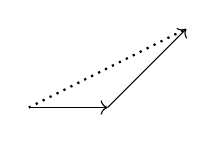
\begin{tikzpicture}
\draw[->] (0, 0) -- (1, 0);
\draw[->] (1,0) -- (2, 1);
\draw[dotted, thick] (0, 0) -- (2,1);
\end{tikzpicture}
\end{center}
Vector addition is commutative \((\vec a + \vec b=\vec b + \vec a)\) and associative \((\vec a + (\vec b +\vec c)=(\vec a + \vec b) +\vec c)\)
\item Multiplication by a scalar \(c\):
\begin{center}
\begin{tabular}{|c|c|c|}\hline
Value of scalar \(c\) & What happens to the magnitude? & What happens to the direction?\\ \hline
\(c>1\) & Magnitude increases & Direction is unchanged\\ \hline
\(0<c<1\) & Magnitude decreases & Direction is unchanged\\ \hline
\(c=-1\) & Magnitude is unchanged & Direction is reversed\\ \hline
\end{tabular}
\end{center}
\item By combining multiplication by -1 and vector addition we can define vector subtraction as \(\vec a - \vec b = \vec a + (-\vec b)\)
\item Projection:
\begin{center}
\begin{tikzpicture}
\draw[->] (0, 0) -- (0, 1.5);
\draw[->] (0, 0) -- (1.5, 0);
\draw[->] (0, 0) -- (1, 1);
\draw[dotted] (0, 1) -- (1, 1);
\draw[dotted] (1, 0) -- (1, 1);
\end{tikzpicture}
\end{center}
The length of \(\vec v\) projected on \(x\) is \(v_x\), likewise the length of \(\vec v\) projected on \(y\) is \(v_y\). If the angle between \(\vec v\) and the \(x\) axis is \(\vartheta\) then \(v_x\) and \(v_y\) can be calculated as:
\[v_x=v\cos\vartheta \quad \text{\&} \quad v_y=v\sin\vartheta\]
It can be seen from the diagram that \(\vec v = v_x\vec{\hat{x}}+v_y\vec{\hat{y}}\)
\end{enumerate}

\section{More Vector operations}

By choosing a different coordinate system one of the components can be 0:
\begin{center}
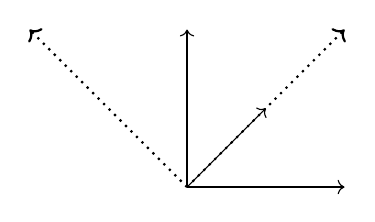
\begin{tikzpicture}
\draw[->] (0, 0) -- (1, 1);
\draw[->] (0, 0) -- (2, 0);
\draw[->] (0, 0) -- (0, 2);
\draw[->, dotted, thick] (0, 0) -- (2, 2);
\draw[->, dotted, thick] (0, 0) -- (-2, 2);
\end{tikzpicture}
\end{center}
If we call the new coordinate system \(x'\) and \(y'\) then it is possible to express the vector \(\vec v\) in terms of \(\vec{\hat{x'}}\) and \(\vec{\hat{y'}}\):
\[\vec v=v_{x'}\vec{\hat{x'}}+v_{y'}\vec{\hat{y'}}=v_{x'}\vec{\hat{x'}}=v\vec{\hat{x'}}\quad \text{as }\vec{\hat{y'}}=\vec 0\]
This shows that the magnitude is not dependant on the coordinate system used, because of this we call it a scalar. The components of the vector are not scalars as they depend on the coordinate system used.

\subsection*{Vector operations revisited}

\begin{itemize}
\item Vector addition:
\begin{center}
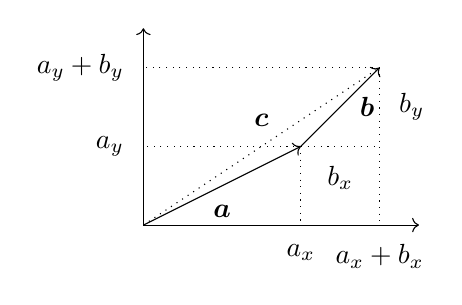
\begin{tikzpicture}
\draw[<->] (3.5, 0) -- (0, 0) -- (0, 2.5);
\draw[->] (0, 0) -- (2, 1);
\node[label=below:{\(\vec a\)}] at (1, .5) {};
\draw[->] (2, 1) -- (3, 2);
\node[label=right:{\(\vec b\)}] at (2.5, 1.5) {};
\draw[dotted] (2,1) -- (2, 0);
\draw[dotted] (2,1) -- (0,1);
\draw[dotted] (3,2) -- (3,0);
\draw[dotted] (3,2) -- (0,2);
\node[label=below:{\(a_x\)}] at (2,0) {};
\node[label=below:{\(a_x+b_x\)}] at (3,0) {};
\node[label=left:{\(a_y\)}] at (0, 1) {};
\node[label=left:{\(a_y+b_y\)}] at (0, 2) {};
\draw[dotted] (2,1) -- (3,1);
\node[label=below:{\(b_x\)}] at (2.5,1) {};
\node[label=right:{\(b_y\)}] at (3,1.5) {};
\draw[dotted] (0,0) -- (3,2);
\node[label=above:{\(\vec c\)}] at (1.5,1) {};
\end{tikzpicture}
\end{center}
\begin{align*}
\vec a &= a_x\vec{\hat{x}}+a_y\vec{\hat{y}}\\
\vec b &= b_x\vec{\hat{x}}+b_y\vec{\hat{y}}\\
\vec c &= c_x\vec{\hat{x}}+c_y\vec{\hat{y}}\\
\vec c&=\vec a+\vec b\\
c_x&=a_x+b_x\\
c_y&=a_y+b_y\\
\vec c&=(a_x+b_y)\vh x +(a_y+b_y)\vh y\\
\vv a +\vv b&=(a_x+b_x)\vh x +(a_y+b_y)\vh y\\
\end{align*}
This works in 3 dimensions as well. If \(\vv v\) and \(\vv u\) are 3-dimensional vectors then: \[\vv v + \vv u=(v_x+u_x)\vh x+(v_y+u_y)\vh y+(v_z+u_z)\vh z\]
\item Scalar multiplication:
\begin{align*}
\vv a&=a_x\vh x+a_y\vh y\\
c\vv a&=c(a_x\vh x+a_y\vh y)\\
c\vv a&=ca_x\vh x+ca_y\vh y
\end{align*}
Multiplication by \(-1\)
\begin{center}
\begin{tikzpicture}
\draw[<->] (2, 0) -- (0, 0) -- (0, 2);
\draw[->] (0,0) -- (1,1);
\draw (-2, 0) -- (0, 0) -- (0, -2);
\node[label=above right:{\(\vv a\)}] at (1,1) {};
\draw[->] (0,0) -- (-1,-1);
\node[label=below left:{\(-\vv a\)}] at (-1,-1) {};
\draw[dotted] (1,0) -- (1,1);
\draw[dotted] (0,1) -- (1,1);
\draw[dotted] (0,-1) -- (-1,-1);
\draw[dotted](-1,0) -- (-1,-1);
\node[label=below:{\(a_x\)}] at (1,0) {};
\node[label=above:{\(-a_x\)}] at (-1,0) {};
\node[label=left:{\(a_y\)}] at (0,1) {};
\node[label=right:{\(a_y\)}] at (0,-1) {};
\end{tikzpicture}
\end{center}

\begin{align*}
\vv a&=a_x\vh x+a_y\vh y\\
-\vv a&=-(a_x\vh x+a_y\vh y)\\
-\vv a&=-a_x\vh x-a_y\vh y
\end{align*}

The negative signs don't mean that the length is negative but that they go in the opposite direction to the direction defined as positive.
\end{itemize}

Calculaing the magnitude:
If \(\vv v\) is a 2-dimensional vector then \(v=|\vv v|=\sqrt{v_x^2+v_y^2}\)
If \(\vv w\) is a 3-dimensional vector then \(w=|\vv w|=\sqrt{w_x^2+w_y^2+w_z^2}\)

\subsection*{Notation}

If \(\vv v\) is an \(n\)-dimensional vector then as we run out of letters for cartesian coordinates it is necessary to use different notation, we call each direction \(e_i\) instead of x, y, z etc.:
\begin{align*}
\vv v&=v_1\vh{e_1}+v_2\vh{e_2}+v_3\vh{e_3}+\cdots+v_n\vh{e_n}\\
&=\sum_{i=1}^nv_i\vh{e_i}\\
&=v_i\vh{e_i}
\end{align*}
The last notation \((v_i\vh{e_i})\) is called Einstein's summation convention. The repeated subscript shows it is a sum.

\section{General Method For Vector Mechanics}

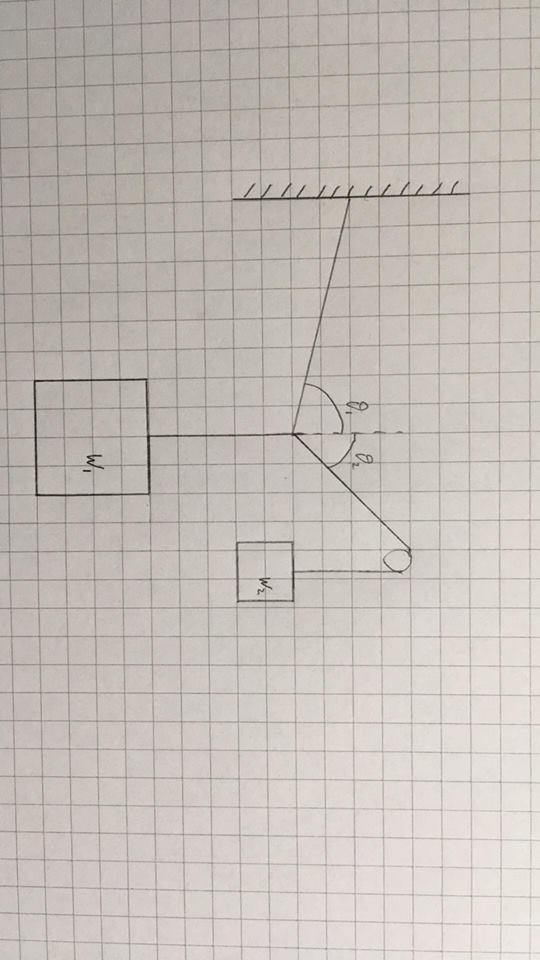
\includegraphics[scale=0.2, angle=90]{Diagram1}

Find \(\vv{w_1}\) in terms of \(\vartheta_1,\vartheta_2\) and \(\vv{w_1}\)

\underline{method:}

\begin{enumerate}
\item Sketch a diagram and draw vectors:

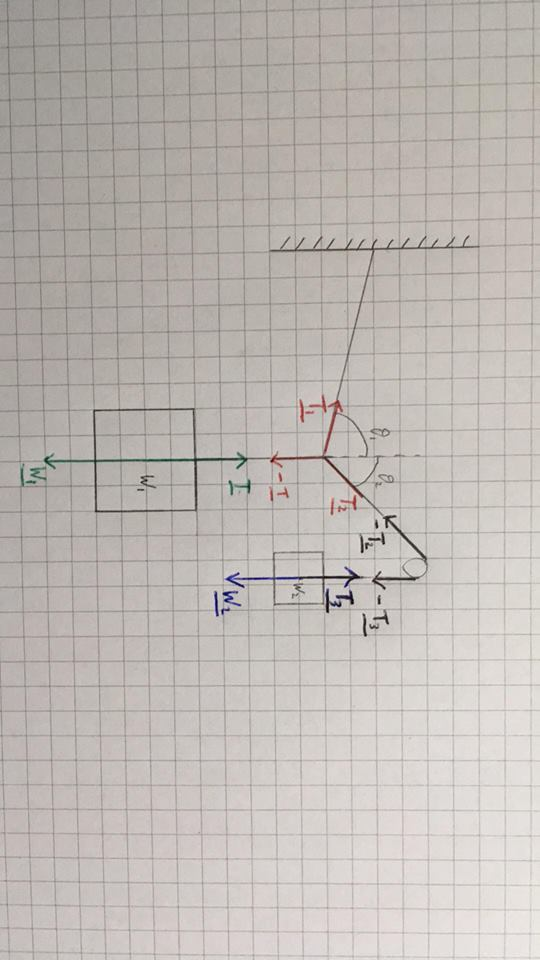
\includegraphics[scale=0.2, angle=90]{Diagram2}

\item Identify any relevant vector equations. In this case we have Newton's 2\(^\text{nd}\) law (NII) and the nature of a pulley to give the equations:
\begin{align*}
\vv{w_1}+\vv T=&\vv 0\tag{2.1}\\
\vv{w_2}+\vv{T_3}=&\vv 0\tag{2.2}\\
\vv{T_1}+\vv{T_2}+(-\vv T)=&\vv 0\tag{2.3}\\
|-\vv{T_2}|=&|-\vv{T_3}|\tag{2.4}
\end{align*}
\item Choose a coordinate frame and draw it on the diagram:

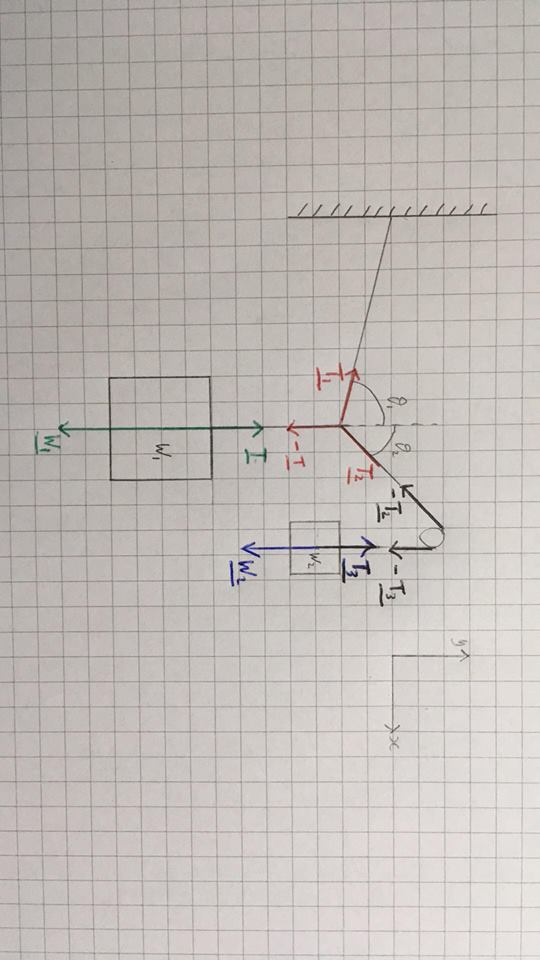
\includegraphics[scale=0.2, angle=90]{Diagram3}

\item Decompose vectors into this coordinate system:
\begin{align*}
\vv{w_1}&=-w_1\vh y\\
\vv{w_2}&=-w_2\vh y\\
\vv T&=T\vh y\\
\vv{T_1}&=-T_1\vh x\sin\vartheta_1+T_1\vh y\cos\vartheta_1\\
\vv{T_2}&=T_2\vh x\sin\vartheta_2+T_2\vh y\cos\vartheta_2\\
\vv{T_3}&=T_3\vh y
\end{align*}
\item Extract the number equations (or component equations) from the vector equations:
\begin{align*}
(2.1)\implies& w_1=T\tag{2.5}\\
(2.2)\implies& w_2=T_3\tag{2.6}\\
(2.3)\implies& T_1\sin\vartheta_1+T_2\sin\vartheta_2=0\tag{2.7}\\
(2.3)\implies& -T+T_1\cos\vartheta_1+T_2\cos\vartheta_2=0\tag{2.8}\\
(2.4)\implies& T_2=T_3\tag{2.9}
\end{align*}
\item Solve:
\begin{align*}
(2.7)\implies T_1&=T_2\frac{\sin\vartheta_2}{\sin\vartheta_1}\\
\intertext{Substituting \(T_1\) in (2.8)}
T&=T_2\left(\frac{\sin\vartheta_2}{\tan\vartheta_1}+\cos\vartheta_2\right)\\
\intertext{(2.6) and (2.9)}
T_2&=T_3=w_2
\end{align*}
Therefore\[w_1=w_2\left[\frac{\sin\vartheta_2}{\tan\vartheta_1}+\cos\vartheta_2\right]\] is the magnitude of \(w_1\) and \(\vv{w_1}=-w_1\vh y\) in the chosen coordinate frame.
\end{enumerate}

\section{Scalar and Vector Products}

\subsection*{Defining new vector operations}

Vectors are invarient under coordinate transformation. To define more vector operations we start by constructing other quantities that share this property. \(|\vv a||\vv b|\) is invarient and so is \(\vartheta\) the angle between \(\vv a\) and \(\vv a\). Combining these it is possible to get:
\[(3.1)\quad ab\cos\vartheta\qquad\&\qquad(3.2)\quad ab\sin\vartheta\]
(3.1) can be interpreted as the magnitude of the projection of \(\vv a\) on \(\vv b\) times the magnitude of \(\vv b\) or the magnitude of the projection of \(\vv b\) on \(\vv a\) times the magnitude of \(\vv a\). We define this as the scalar (dot) product of \(\vv a\) and \(\vv b\):
\[\vv a\cdot\vv b=|\vv a||\vv b|\cos\vartheta\]
Note that the dot product is commutative:
\[\vv a\cdot\vv b\equiv\vv b\cdot\vv a\]

(3.2) can be interpreted as the area of the parallelogram formed by \(\vv a\) and \(\vv b\). Surfaces can be represented by a vector giving the area and which side of the surface. We introduce the normal vector \(\vh n\) which is perpendicular to the surface at all points and points out of the side that we are interested in. We define this as the vector (cross) product of \(\vv a\) and \(\vv b\):
\[\vv a\times\vv b=|\vv a||\vv b|\vh n\sin\vartheta\]

Note that the cross product is not commutative:
\[\vv a\times\vv b=-\vv b\times\vv a\]

\subsection*{Algebraic representation of the scalar product}


\[\vv a=a_1\vh{e_1}+a_2\vh{e_2}\quad\&\quad\vv b=b_1\vh{e_1}+b_2\vh{e_2}\]
\[\vv a\cdot\vv b=(a_1\vh{e_1}+a_2\vh{e_2})\cdot(b_1\vh{e_1}+b_2\vh{e_2})\]
Since \(a_1, a_2, b_1\) and \(b_2\) are scalars the dot product turns into normal multiplication for them. Expanding the brackets gives:
\[\vv a\cdot\vv b=a_1b_1(\ve1\cdot\ve1)+a_1b_2(\ve1\cdot\ve2)+a_2b_1(\ve2\cdot\ve1)+a_2b_2(\ve2\cdot\ve2)\]

\[e_1=e_2=1 \quad\&\quad\vartheta=\pi\]
\[\ve1\cdot\ve1=\ve2\cdot\ve2=1\cdot1\cos0=1\]
\[\ve1\cdot\ve2=\ve2\cdot\ve1=1\cdot1\cos\pi=0\]
\[\therefore \vv a\cdot\vv b=a_1b_1+a_2b_2\]

This result is true in all dimensions. In general:

\begin{center}
\boxed{a_i\ve i\cdot b_i\ve i=a_ib_i=ab\cos\vartheta}
\end{center}

Several useful results come from this:
\begin{itemize}
\item The angle between two vectors \(\vv a\) and \(\vv b\) can be calculated using the following formula:
\[\vartheta=\arccos\frac{\vv a\cdot\vv b}{ab}\]
\item If \(\vv a\cdot\vv b=0\) then either \(a\) and/or \(b\) is \(\vv0\) or \(\vv a\) and \(\vv b\) are perpendicular. 
\end{itemize}

\section{Properties of Scalar and Vector Products}


Distributive law of the dot product:
\[\vv a\cdot(\vv b+\vv c)\equiv\vv a\cdot\vv b+\vv a\cdot\vv c\]

\subsection*{Vector product}

Distributive law of the cross product:

\[\vv a\times(\vv b+\vv c)\equiv\vv a\times\vv b+\vv a\times\vv c\]

\subsection*{Algebraic representation of the vector product}

Let \(\vv a=a_1\ve1+a_2\ve2+a_3\ve3\) and \(\vv b=b_1\ve1+b_2\ve2+b_3\ve3\)


\[\vv a\times \vv b=(a_1\ve1+a_2\ve2+a_3\ve3)\times(b_1\ve1+b_2\ve2+b_3\ve3)\]
\begin{multline*}
=a_1b_1(\ve1\times\ve1)+a_1b_2(\ve1\times\ve2)+a_1b_3(\ve1\times\ve3)+a_2b_1(\ve2\times\ve1)+a_2b_2(\ve2\times\ve2)+a_2b_3(\ve2\times\ve3)\\+a_3b_1(\ve3\times\ve1)+a_3b_2(\ve3\times\ve2)+a_3b_3(\ve3\times\ve3)
\end{multline*}
\[\ve1\times\ve1=\ve2\times\ve2=\ve3\times\ve3=1\cdot1\sin\frac{\pi}{2}\vh n=0\]
\[\ve1\times\ve2=\ve3,\quad\ve1\times\ve3=-\ve2,\quad\ve2\times\ve1=-\ve3,\quad\ve2\times\ve3=\ve1,\quad\ve3\times\ve1=\ve2,\quad\ve3\times\ve2=-\ve1\]
\[\vv a\times\vv b=a_1b_2\ve3-a_1b_3\ve2-a_2b_1\ve3+a_2b_3\ve1+a_3b_1\ve2-a_3b_2\ve1\]
\[=\ve1(a_2b_3-a_3b_2)+\ve2(a_3b_1-a_1b_3)+\ve3(a_1b_2-a_2b_1)\]

\begin{itshape}
The following is not on the mfp2 course:

For some \(i,j,k\in\{1,2,3\}\):
\[\ve i\cdot\ve j=\delta_{ij}\]
\(\delta_{ij}\) is called Kroneker's delta and has the property that:

\[\delta_{ij}=
   \begin{cases} 
      1& \text{\emph{if} } i=j \\
      0& \text{\emph{if} } i\ne j \\
   \end{cases}\]

\[\ve i\times\ve j=\ve k\varepsilon_{ijk}\]
\(\varepsilon_{ijk}\) is called the Levi-Civita symbol and has the property that:

\[\varepsilon_{ijk}=
   \begin{cases}
      1& \text{\emph{for an even permutation}}\\
      -1& \text{\emph{for an odd permutation}}\\
      0& \text{\emph{for all other cases}}
   \end{cases}\]

An even permutation is one where that is formed from cycling through 1,2,3 in that order and an odd permutation cycles through 3,2,1.
\end{itshape}

If \(\vv a\times\vv b=0\) then either \(\vv a\) or \(\vv b =\vv 0\) or they are parallel.

\[\vv a\cdot\vv a=a^2\cos 0=a^2\]
We can use this to 'remove' all vectors and equate coefficients since if \(\vv a=a_1\ve1+a_2\ve2+a_3\ve3\) then \(\vv a\cdot\ve1=a_1\).

\subsection*{Vector identities}

\begin{itemize}
\item Scalar triple product:
\[\vv a\cdot(\vv b\times\vv c)=\vv b\cdot(\vv c\times \vv a)=\vv c\cdot(\vv a\times\vv b)=\text{Volume of the parallelipiped with CSA \(|\vv b\times\vv c|\) and side length \(a\)}\]
\item Vector triple product (bac-cab rule):
\[\vv a\times(\vv b\times\vv c)=\vv b(\vv a\cdot c)-\vv c(\vv a\cdot\vv b)\]
Since for cartesian coordinates all directions are indistinguishable then this result can be proved to be true for the \(\ve1\) component and that implies it is true for all components. To do this we dot product both sides with \(\ve1\):
\[\ve1\cdot(\vv a\times(\vv b\times\vv c))=\ve1\cdot(\vv b(\vv a\cdot c)-\vv c(\vv a\cdot\vv b))\]
\end{itemize}

\part{Determinants}
\section{Vector Product as a Determinant}

\[\vv a\times\vv b=\ve 1 (a_2b_3-a_3b_2)+\ve 2 (a_3b_1-a_1b_3)+\ve 3 (a_1b_2-a_2b_1)=
\begin{vmatrix}
\ve1 & \ve2 & \ve3\\
a_1 & a_2 & a_3\\
b_1 & b_2 & b_3\\
\end{vmatrix}
\]
We call this the determinant of the matrix 
\(\left[
\begin{smallmatrix}
\ve1 & \ve2 & \ve3\\
a_1 & a_2 & a_3\\
b_1 & b_2 & b_3\\
\end{smallmatrix}
\right]\).
We define the determinant of a \(2\times2\) matrix as:
\[\begin{vmatrix}
a & b\\
c & d
\end{vmatrix}
\triangleq ad-bc\]

\(3\times3\) determinant by Pierre sarrus' rule:

The following is known as an ``augmented" matrix:
\[A=
\begin{array}{|ccc|cc|}
a_1 & a_2 & a_3 & a_1 & a_2\\
b_1 & b_2 & b_3 & b_1 & b_2\\
c_1 & c_2 & c_3 & c_1 & c_2
\end{array}
\]
Take the product of every diagonal that has an \(a_i,b_i\) and \(c_i\) From both top left to bottom right and top right to bottom left. If it is right to left it gets a positive sign and if it is left to right it gets a negative sign. The sum of these produccts is \(\det A\).

Generalisation to \(n\times n\) matrix \((n\in\bb N)\) by Pierre Laplace:

Let \(A\) be a matrix size \(n\times n\) where \(A\) is composed of elements \(a_{ij}\) where \(a_{ij}\) is in row \(i\) and column \(j\):
\[
\begin{bmatrix}
a_{11} & a_{12} & \cdots & a_{1n}\\
a_{21} & a_{22} & \cdots & a_{2n}&\\
\vdots &\vdots & \ddots &\vdots &\\
a_{n1} & a_{n2} & \cdots & a_{nn}
\end{bmatrix}
\]

Then the determinant of \(A\) is given as:
\[\det A=\sum_{i=1}^na_{ij}C_{ij}\]
In this \(C_{ij}\) is the cofactor of the element \(a_{ij}\) and it is defined as:
\[C_{ij}=(-1)^{i+j}M_{ij}\]
Where \(M_{ij}\) is the minor of element \(a_{ij}\) which is the determinant of the \((n-1)\times(n-1)\) matrix made by removing row \(i\) and column \(j\).

This formula allows any value of \(j\) to be picked and then is computed for all values of \(i\). The formula also holds if you pick a value of \(i\) and then replace all \(i\)s in the formula with \(j\)s and compute it that way. We say that the matrix is expanded/reduced by row \(i\) or column \(j\)

\begin{example}
Compute the following determinant by Lapalce expansion about the first row:
\[
\begin{vmatrix}
a_{11} & a_{12} & a_{13}\\
a_{21} & a_{22} & a_{23}\\
a_{31} & a_{32} & a_{33}
\end{vmatrix}
\]
\[=a_{11}(-1)^{1+1}
\begin{vmatrix}
a_{22} & a_{23}\\
a_{32} & a_{33}
\end{vmatrix}
+a_{12}(-1)^{1+2}
\begin{vmatrix}
a_{21} & a_{23}\\
a_{31} & a_{33}
\end{vmatrix}
+a_{13}(-1)^{1+3}
\begin{vmatrix}
a_{21} & a_{22}\\
a_{31} & a_{32}
\end{vmatrix}
\]
\[=a_{11}(a_{22}a_{33}-a_{23}a_{23}a_{32})-a_{12}(a_{21}a_{33}-a_{23}a_{31})+a_{13}(a_{21}a_{32}-a_{22}a_{31})\]
\end{example}
\subsection*{Scalar triple product}

\[\vv a\cdot(\vv b\times\vv c)\]
\[=(a_1\ve1+a_2\ve2+a_3\ve3)\cdot\left[\ve1
\begin{vmatrix}
b_2 & b_3\\
c_2 & c_3
\end{vmatrix}
-\ve2
\begin{vmatrix}
b_1 & b_3\\
c_1 & c_3
\end{vmatrix}
+\ve3
\begin{vmatrix}
b_1 & b_2\\
c_1 & c_2
\end{vmatrix}
\right]\]
\[a_1
\begin{vmatrix}
b_2 & b_3\\
c_2 & c_3
\end{vmatrix}
-a_2
\begin{vmatrix}
b_1 & b_3\\
c_1 & c_3
\end{vmatrix}
+a_3
\begin{vmatrix}
b_1 & b_2\\
c_1 & c_2
\end{vmatrix}\]
\[=
\begin{vmatrix}
a_1 & a_2 & a_3\\
b_1 & b_2 & b_3\\
c_1 & c_2 & c_3
\end{vmatrix}
\]

\section{General Properties of Determinants}

Illustrated by the \(3\times3\) matrix \(A\):
\[\det A=\vv a\cdot(\vv b\times\vv c)=
   \begin{vmatrix}
      a_1 & a_2 & a_3\\
      b_1 & b_2 & b_3\\
      c_1 & c_2 & c_3
   \end{vmatrix}
\]

\begin{enumerate}

   \item Writing rows as columns leaves the value of the determinant unchanged:
      \[
      \begin{vmatrix}
         a_1 & a_2 & a_3\\
         b_1 & b_2 & b_3\\
         c_1 & c_2 & c_3
      \end{vmatrix}
      = a_1(b_2c_3-b_3c_2)-a_2(b_1c_3-b_3c_1)+a_3(b_1c_2-b_2c_1)\]
      \[= a_1b_2c_3-a_1b_3c_2-a_2b_1c_3+a_2b_3c_1+a_3b_1c_2-a_3b_2c_1\]
      \[=a_1(b_2c_3-b_3c_2)-b_1(a_2c_3-a_3c_2)+c_1(a_2b_3-b_2a_3)=
      \begin{vmatrix}
         a_1 & b_1 & c_1\\
         a_2 & b_2 & c_2\\
         a_3 & b_3 & c_3
      \end{vmatrix}
      =\det A\]

   \item If each element of a row or column of a determinant is multiplied by a number \(\lambda\) then the value of the determinant is multiplied by lambda:
      \[
      \begin{vmatrix}
         \lambda a_1 & \lambda a_2 & \lambda a_3\\
         b_1 & b_2 & b_3\\
         c_1 & c_2 & c_3
      \end{vmatrix}
      =(\lambda\vv a)\cdot(\vv b\times\vv c)=\lambda(\vv a\cdot(\vv b\times\vv c))=\lambda\det A\]

   \item The determinant is zero when:
      \begin{itemize}
         \item Any one row or column has only zero as elements:
            \[
            \begin{vmatrix}
               0 & 0 & 0\\
               b_1 & b_2 & b_3\\
               c_1 & c_2 & c_3
            \end{vmatrix}
            =\vv 0\cdot(\vv b\times\vv c)=0\]
         \item Any of the rows or columns are identcal:
            \[
            \begin{vmatrix}
               a_1 & a_2 & a_3\\
               b_1 & b_2 & b_3\\
               b_1 & b_2 & b_3
            \end{vmatrix}
            =\vv a\cdot(\vv b\times\vv b)=0\]
         \item Any row or column is a multiple of another row or column:
            \[
            \begin{vmatrix}
               a_1 & a_1 & a_2\\
               b_1 & b_2 & b_3\\
               \lambda b_1 & \lambda b_2 & \lambda b_3
            \end{vmatrix}
            =\vv a\cdot(\vv b\times(\lambda\vv b))=\lambda(\vv a\cdot(\vv b\times\vv b))=0\]
      \end{itemize}

   \item If two consecutive rows or columns are interchanged then the sign reverses:
      \[
      \begin{vmatrix}
         a_1 & a_2 & a_3\\
         b_1 & b_2 & b_3\\
         c_1 & c_2 & c_3
      \end{vmatrix}
      =\vv a\cdot(\vv b\times\vv c)=-\vv a\cdot(\vv c\times\vv b)=-\vv b\cdot(\vv a\times\vv c)=
      \begin{vmatrix}
         b_1 & b_2 & b_3\\
         a_1 & a_2 & a_3\\
         c_1 & c_2 & c_3
      \end{vmatrix}
      \]
   \item The value of the determinant is unchanged if, to each element in a row or column, you add \(\lambda\) times the corresponding element of another row or column:
      \begin{multline*}
         \begin{vmatrix}
            a_1+\lambda b_1 & a_2+\lambda b_2 & a_3 +\lambda b_3\\
            b_1 & b_2 & b_3\\
            c_1 & c_2 & c_3
         \end{vmatrix}
         =(\vv a+\lambda\vv b)\cdot(\vv b\times\vv c)=\vv a\cdot(\vv b\times\vv c)+\lambda\vv b\cdot(\vv b\times\vv c)=\\\vv a\cdot(\vv b\times\vv c)+\lambda\vv c\cdot(\vv b\times\vv b)=\vv a\cdot(\vv b\times\vv c)=
         \begin{vmatrix}
            a_1 & a_2 & a_3\\
            b_1 & b_2 & b_3\\
            c_1 & c_2 &c_3
         \end{vmatrix}
      \end{multline*}
\end{enumerate}

\subsection*{Vectors}

In 3D three vectors \(\vv a,\vv b\) and \(\vv c\) are linearly independant if, for some constants \(\alpha,\beta\) and \(\gamma\) the equation \(\alpha\vv a+\beta\vv b+\gamma\vv c=\vv 0\) has only one solution which is \(\alpha=\beta=\gamma=0\)

This is the same as saying \(\vv a\cdot(\vv b\times\vv c)=\det A\ne0\).

If \(\vv a,\vv b\) and \(\vv c\) are linearly independant then they can be combined linearly to express any 3D vector.

\begin{example}
Express \(\vv w=w_1\ve1+w_2\ve2+w_3\ve3\) as a linear combination of \(\vv a=(1,1,1),\vv b=(1,1,0)\) and \(\vv c=(1,0,0)\)

First check that they are linearly independant:
\[\vv a\cdot(\vv b\times\vv c)=
\begin{vmatrix}
1 & 1 & 1\\
1 & 1 & 0\\
1 & 0 & 0
\end{vmatrix}
=-1\ne0\]
so they are linearly independant.

\[\vv w=\alpha\vv a+\beta\vv b+\gamma\vv c\]
\begin{align*}
w_1=\alpha + \beta +\gamma\tag{6.1}\\
w_2=\alpha + \beta \tag{6.2}\\
w_3=\alpha\qquad&\tag{6.3}
\end{align*}
\[(6.3)\implies\alpha=w_3\]
\[(6.2)-(6.3)\implies\beta=w_2-w_3\]
\[(6.1)-(6.2)\implies\gamma=w_1-w_2\]
\[\vv w=w_3\vv a+(w_2-w_3)\vv b+(w_1-w_2)\vv c\]
\end{example}
\section{Physics Applications}

\subsection*{Electrostatics}

Coulomb's law:
\[\vv F_{12}=k\frac{Q_1Q_2}{|\vv r_1-\vv r_2|^3}(\vv r_1-\vv r_2)\]

\begin{center}
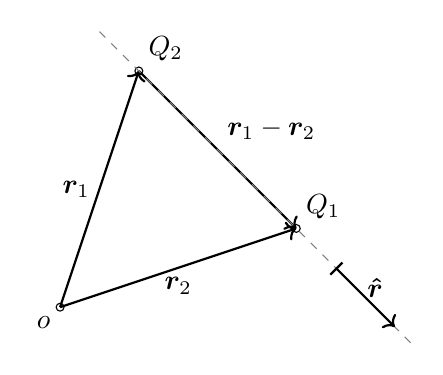
\begin{tikzpicture}
\draw (1,3) circle [radius=0.05];
\draw (3,1) circle [radius=0.05];
\draw (0,0) circle [radius=0.05];
\draw [->, thick] (0,0) -- (1,3);
\draw [->, thick] (0,0) -- (3,1);
\node [below left] at (0,0) {\(o\)};
\node [above right] at (1,3) {\(Q_2\)};
\node [above right] at (3,1) {\(Q_1\)};
\draw [->, thick] (1,3) -- (3,1);
\node [left] at (0.5,1.5) {\(\vv r_1\)};
\node [below] at (1.5,0.5) {\(\vv r_2\)};
\node [above right] at (2,2) {\(\vv r_1-\vv r_2\)};
\draw [dashed, gray] (0.5,3.5) -- (4.5,-0.5);
\draw [|->, thick] (3.5,0.5) -- (4.25,-0.25);
\node [above] at (4,0) {\(\vh r\)};
\end{tikzpicture}
\end{center}
\[\vh r=\frac{\vv r_1-\vv r_2}{|\vv r_1-\vv r_2|}\]
\[\vv F_{12}=k\frac{Q_1Q_2}{|\vv r_1-\vv r_2|^2}\vh r\]

\begin{example}
Three positive charges \(Q_1,Q_2\) and \(Q_3\) are intially in the corners of a right angle triangle as shown:

\begin{center}
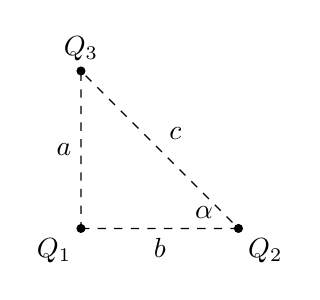
\begin{tikzpicture}
\draw [fill=black] (0,2) circle [radius=0.05];
\draw [fill=black] (2,0) circle [radius=0.05];
\draw [fill=black] (0,0) circle [radius=0.05];
\draw [dashed] (0,0) -- (2,0) -- (0,2) -- (0,0);
\node [below left] at (0,0) {\(Q_1\)};
\node [below right] at (2,0) {\(Q_2\)};
\node [above] at (0,2) {\(Q_3\)};
\node [above right] at (1,1) {\(c\)};
\node [below] at (1,0) {\(b\)};
\node [left] at (0,1) {\(a\)};
\node [above left] at (1.8,0) {\(\alpha\)};
\end{tikzpicture}
\end{center}

Find the resultant force \(\vv R\) on \(Q_3\):

Step one - Draw the vectors:

\begin{center}
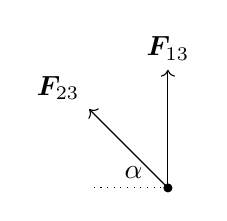
\begin{tikzpicture}
\draw [fill=black] (0,0) circle [radius=0.05];
\draw [->] (0,0) -- (0,1.5);
\draw [->] (0,0) -- (-1,1);
\node [above] at (0,1.5) {\(\vv F_{13}\)};
\node [above left] at (-1,1) {\(\vv F_{23}\)};
\draw [dotted] (0,0) -- (-1,0);
\node [above left] at (-0.2,0) {\(\alpha\)};
\end{tikzpicture}
\end{center}

Step 2 - Identify vector equations:

\[\vv R=\vv F_{13}+\vv F_{23}\]

Step 3 - Choose a coordinate system:

\begin{center}
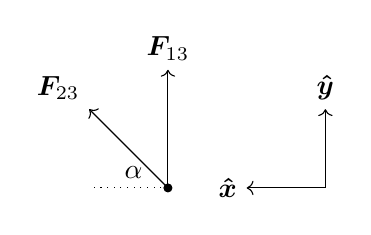
\begin{tikzpicture}
\draw [fill=black] (0,0) circle [radius=0.05];
\draw [->] (0,0) -- (0,1.5);
\draw [->] (0,0) -- (-1,1);
\node [above] at (0,1.5) {\(\vv F_{13}\)};
\node [above left] at (-1,1) {\(\vv F_{23}\)};
\draw [dotted] (0,0) -- (-1,0);
\node [above left] at (-0.2,0) {\(\alpha\)};
\draw [<->] (1,0) -- (2,0) -- (2,1);];
\node [left] at (1,0) {\(\vh x\)};
\node [above] at (2,1) {\(\vh y\)};
\end{tikzpicture}
\end{center}

Step 4 - Decompose into coordinates:

\[\vv F_{13}=F_{13}\vh y=k\frac{Q_1Q_3}{a^2}\vh y\]
\[\vv F_{23}=F_{23}\cos\alpha\vh x+F_{23}\sin\alpha\vh y=k\frac{Q_2Q_3}{c^2}(\cos\alpha\vh x+\sin\alpha\vh y)\]
\[\vv R=kQ_3\left[\frac{Q_2}{c^2}\cos\alpha\vh x+\left(\frac{Q_1}{a^2}+\frac{Q_2}{c^2}\sin\alpha\right)\vh y\right]\]
\end{example}
\subsection*{Torque \(\vv\tau\) or moment \(\vv M_o\)}

\begin{center}
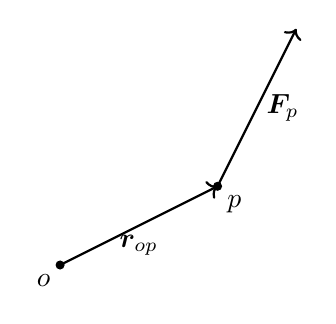
\begin{tikzpicture}
\draw [fill=black] (0,0) circle [radius=0.05];
\draw [fill=black] (2,1) circle [radius=0.05];
\draw [->, thick] (0,0) -- (2,1);
\draw [->, thick] (2,1) -- (3,3);
\node [below left] at (0,0) {\(o\)};
\node [below right] at (2,1) {\(p\)};
\node [right] at (2.5,2) {\(\vv F_p\)};
\node [below] at (1,0.5) {\(\vv r_{op}\)};
\end{tikzpicture}
\end{center}

\(\vv F_p\) is a force acting through point \(p\). The moment about \(o\) is given by:
\[\vv M_o=\vv r_{op}\times\vv F_p\]
\(\vv M_o\) is perpendicular to both \(\vv r_{op}\) and \(\vv F_p\).

If \(\vv M_o=\vv 0\) then there is no rotation and, \(\vv r_{op}\) and \(\vv F_p\) are colinear.

But what if, instead of \(p\), we picked a different point on the line of action of the force?

\begin{center}
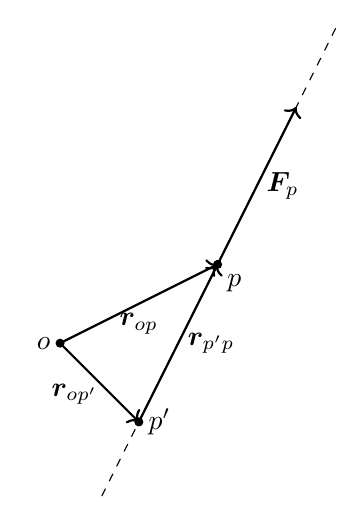
\begin{tikzpicture}
\draw [fill=black] (0,0) circle [radius=0.05];
\draw [fill=black] (2,1) circle [radius=0.05];
\draw [->, thick] (0,0) -- (2,1);
\draw [->, thick] (2,1) -- (3,3);
\node [left] at (0,0) {\(o\)};
\node [below right] at (2,1) {\(p\)};
\node [right] at (2.5,2) {\(\vv F_p\)};
\node [below] at (1,0.5) {\(\vv r_{op}\)};
\draw [dashed] (3.5,4) -- (0.5,-2);
\draw [fill=black] (1,-1) circle [radius=0.05];
\node [right] at (1,-1) {\(p'\)};
\draw [->, thick] (0,0) -- (1,-1);
\node [below left] at (0.6,-0.4) {\(\vv r_{op'}\)};
\draw [->, thick] (1,-1) -- (2,1);
\node [right] at (1.5,0) {\(\vv r_{p'p}\)};
\end{tikzpicture}
\end{center}

From the diagram it can be seen that:
\[\vv r_{op}=\vv r_{op'}+\vv r_{p'p}\]
\[\vv M_o=\vv r_{op}\times\vv F_p=(\vv r_{op'}+\vv r_{p'p})\times\vv F_p=\vv r_{op'}\times\vv F_p+\vv r_{p'p}\times\vv F_p\]
However from the diagram we know that \(\vv r_{p'p}\) and \(\vv F_p\) are colinear so \(\vv r_{p'p}\times\vv F_p=\vv 0\) therefore the moment about \(o\) is given by:
\[\vv r_{op'}\times\vv F_p\]
So as long as point \(p\) is on the line of action of the force the formula is the same.

If instead we want to find the moment \(\vv M_l\) about some line \(l\):

\begin{center}
\begin{tikzpicture}[scale=0.75]
\draw [fill=black] (0,0) circle [radius=0.05];
\draw [->, thick] (0,0) -- (4,1);
\draw [->, thick] (4,1) -- (5,4);
\draw [dashed] (-2,2) -- (2,-2);
\node [above left] at (-2,2) {\(l\)};
\node [below left] at (0,0) {\(o\)};
\node [below] at (2,0.5) {\(\vv r_{op}\)};
\node [right] at (4.5,3) {\(F_p\)};
\end{tikzpicture}
\end{center}

First find \(\vv M_o\) where \(o\) is a point on line \(l\):
\[\vv M_o=\vv r{op}\times\vv F_p\]
Next find the projection of \(\vv M_o\) along line \(l\):
\[\vv M_o\cdot\vh l=M_l\]
\[\vv M_l=M_l\vh l=(M_o\cdot\vh l)\vh l\]

But what if we had chosen a different point \(o'\) on \(l\)?

\begin{center}
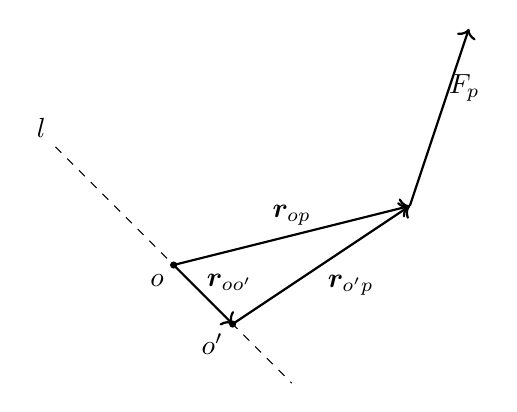
\begin{tikzpicture}[scale=0.75]
\draw [fill=black] (0,0) circle [radius=0.05];
\draw [->, thick] (0,0) -- (4,1);
\draw [->, thick] (4,1) -- (5,4);
\draw [dashed] (-2,2) -- (2,-2);
\node [above left] at (-2,2) {\(l\)};
\node [below left] at (0,0) {\(o\)};
\node [above] at (2,0.5) {\(\vv r_{op}\)};
\node [right] at (4.5,3) {\(F_p\)};
\draw [fill=black] (1,-1) circle [radius=0.05];
\draw [->, thick] (1,-1) -- (4,1);
\node [below] at (3,0) {\(\vv r_{o'p}\)};
\draw [->, thick] (0,0) -- (1,-1);
\node [below left] at (1,-1) {\(o'\)};
\node [above right] at (0.4,-0.6) {\(\vv r_{oo'}\)};
\end{tikzpicture}
\end{center}

\[\vv M_l=\vh l\cdot\vv M_o=\vh l\cdot(\vv r_{op}\times\vv F_p)=\vh l\left[(\vv r_{oo'}+\vv r_{o'p})\times\vv F_p\right]=\vh l\cdot(\vv r_{oo'}\times \vv F_p)+\vh l\cdot(\vv r_{o'p}\times\vv F_p)\]
\((\vv r_{oo'}\times\vv F_p)\) is perpendicular to \(\vh l\) as \(\vv r_{oo'}\) is parallel to \(\vh l\) so \(\vh l\cdot(\vv r_{oo'}\times\vv F_p)=0\). Therefore the moment about line \(l\) is given by:
\[\vv M_l=\vh l\cdot(\vv r_{op}\times\vv F_p)=\vh l\cdot(\vv r_{o'p}\times\vv F_p)\]
So the point on the line doesn't matter.

\part{Matrices}
\section{Matrices introduction}

We will introduce a way of representing the cartesian components of \(\vv a,\vv b\) and \(\vv c\):
\[
\begin{pmatrix}
a_1 & a_2 & a_3\\
b_1 & b_2 & b_3\\
c_1 & c_2 & c_3\\
\end{pmatrix}
\]
We call this a matrix. A matrix is an ordered list of elements. A marix is of order rows\(\times\)columns or \(m\times n\). The example above is \(3\times3\). A matrix is denoted by a letter eg. \(M=\left(
\begin{smallmatrix}
a & b\\
c & d
\end{smallmatrix}
\right)\). Sometimes it is double underlined \(\underline{\underline{M}}\).

In general a matrix of order \(m\times n\) with elements \(a_{ij}\) where \(i\) is row number and \(j\) is column number \(i,j\in\bb N\) and \(i\le m,j\le n\) will look like this:
\[M=
\begin{pmatrix}
a_{11} & a_{12} & \cdots & a_{1n}\\
a_{21} & a_{22} & \cdots & a_{2n}\\
\vdots & \vdots & \ddots & \vdots\\
a_{m1} & a_{m2} & \cdots & a_{mn}
\end{pmatrix}
\]

\begin{enumerate}
\item Matrices have no algebraic value
\item We define the zero matrix as an \(m\times n\) matrix with all elements equal to 0. That is \(a_{ij}=0\, \A i,j\):
\[
\begin{pmatrix}
0
\end{pmatrix}
,\qquad
\begin{pmatrix}
0 & 0\\
0 & 0
\end{pmatrix}
,\qquad
\begin{pmatrix}
0 & 0 & 0\\
0 & 0 & 0\\
0 & 0 & 0
\end{pmatrix}
\]
\item We define a square matrix as a matrix order \(n\times n\). Square matrices have several special properties, eg they ahave a determinant.
\item If a square matrix has all elemets as 0 except the elements along the leading diagonal then it is called a diagonal matrix. That is a diagonal matrix has elements \(a_{ij}=0\) if \(i\ne j\):
\[
\begin{pmatrix}
1
\end{pmatrix}
,\qquad
\begin{pmatrix}
1 & 0\\
0 & 2
\end{pmatrix}
,\qquad
\begin{pmatrix}
1 & 0 & 0\\
0 & 2 & 0\\
0 & 0 & 3
\end{pmatrix}
\]
\item The identity matrix is a diagonal matrix with all elements on the leading diagonal equal to 1. It is denoted \(\mathds 1\) or \(I\). A subscript number is sometimes added to show the number of rows:
\[I_1=
\begin{pmatrix}
1
\end{pmatrix}
,\qquad I_2=
\begin{pmatrix}
1 & 0\\
0 & 1
\end{pmatrix}
,\qquad I_3=
\begin{pmatrix}
1 & 0 & 0\\
0 & 1 & 0\\
0 & 0 & 1
\end{pmatrix}
\]

\item Matrix equations - Two matrices are only equal if they are identical element by element (that is \(a_ij=b_ij\,\A i,j\). As a result of this both matrices must be of the same order to be compared. This means that two matrices being equal encodes a lot of information:
\[
\begin{pmatrix}
a & b & c\\
x & y & z
\end{pmatrix}
=
\begin{pmatrix}
1 & 2 & 3\\
4 & 5 & 6
\end{pmatrix}
\iff a=1,\,b=2,\,c=3,\,x=4,\,y=5,\,z=6\]
\item Multiplying every element of a matrix by a constant is the same as multiplying the whole matrix by that constant:
\[\lambda
\begin{pmatrix}
a & b & c\\
x & y &z\\
\alpha & \beta & \gamma
\end{pmatrix}
=
\begin{pmatrix}
\lambda a & \lambda b & \lambda c\\
\lambda x & \lambda y &\lambda z\\
\lambda\alpha & \lambda\beta & \lambda\gamma
\end{pmatrix}
\]
\end{enumerate}

\section{Matrix Properteis}

\begin{enumerate}
\setcounter{enumi}{7}
\item To add two matrices they must be of the same order and then just add the corresponding elements. That is the new matrix will have elemnts \(a_{ij}+b_{ij}\):
\[
\begin{pmatrix}
a & b & c\\
d & e & f\\
g & h & i
\end{pmatrix}
+
\begin{pmatrix}
\alpha & \beta & \gamma\\
\delta & \varepsilon & \zeta\\
\eta & \vartheta & \iota
\end{pmatrix}
=
\begin{pmatrix}
a+\alpha & b+\beta & c+\gamma\\
d+\delta & e+\varepsilon & f+\zeta\\
g+\eta & h+\vartheta & i+\iota
\end{pmatrix}
\]
\item If we interchange rows and columns of matrix \(M\) (so that \(a_{ij}\longrightarrow a_{ji}\)) then we get the transposed matrix \(M^T\):
\[M=
\begin{pmatrix}
a & b & c\\
d & e & f
\end{pmatrix}
\iff M^T=
\begin{pmatrix}
a & d\\
b & e\\
c & f
\end{pmatrix}
\]
If we have a vector \(\vv v=v_1\ve1+v_2\ve2+v_3\ve3\) then we can write it as a column matrix and by transposing a row matrix:
\[v=
\begin{pmatrix}
v_1\\ v_2\\ v_3
\end{pmatrix}
\qquad v^T=
\begin{pmatrix}
v_1 & v_2 & v_3
\end{pmatrix}
\]
\item Matrix product - The row by column matrix product of \(A\) and \(B\) is \(AB\)
\[A=
\begin{pmatrix}
a_1 & a_2\\
b_1 & b_2
\end{pmatrix}
,\qquad B=
\begin{pmatrix}
c_1 & d_1\\
c_2 & d_2
\end{pmatrix}
\]
This can be viewed as two row and two column vectors.
\[AB=
\begin{pmatrix}
a_1 & a_2\\
b_1 & b_2
\end{pmatrix}
\begin{pmatrix}
c_1 & d_1\\
c_2 & d_2
\end{pmatrix}
=
\begin{pmatrix}
\vv a\cdot \vv c & \vv a\cdot \vv d\\
\vv b \cdot \vv c & \vv b\cdot \vv d
\end{pmatrix}
=
\begin{pmatrix}
a_1c_1+a_2c_2 & a_1 d_1+a_2d_2\\
b_1c_1+b_2c_2 & b_1d_1+b_2d_2
\end{pmatrix}
\]
For the product \(AB\) to exist matrices \(A\) and \(B\) must have orders \(m\times p\) and \(p\times n\) respectively and the resulting matrix will be order \(m\times n\).

Matrix multiplication is not commutative \((AB\ne BA)\) but it is associative \((A(BC)=(AB)C)\) and distributive over addition \((A(B+C)=AB+AC\ne BA+CA=(B+C)A)\) 

\item For a square matrix \(M\) if \(AM=MA=I\) then we say that \(A\) is the inverse of \(M\) denoted \(M^{-1}\). If \(\det M=0\) then \(M^{-1}\) doesn't exist. This is useful for solving matrix equations as it allows us to get rid of matrices without matrix division:
\[\vv r=(x,y,z)\]
\[M\vv r=\vv k\]
Where \(\vv k\) is a constant vector eg \(\vv k=(a,b,c)\)
\[M^{-1}M\vv r=M^{-1}\vv k\]
\[I\vv r=M^{-1}\vv k\]
\[\vv r=M^{-1}\vv k\]
\end{enumerate}

A square matrix \(A\) of order \(n\times n\) can be denoted \(A_n\)

Every square matrix has an associated determinant \(\det A_n\)

\subsection*{Characteristic polynomial}

Every square matrix \(A_n\) has a characteristic polynomial \(p(\lambda)\) which is defined as
\[p(\lambda)\triangleq\det(\lambda I_n-A_n)\]

\begin{example}
\[A_n=
\begin{pmatrix}
4 & 3\\
5 & 2
\end{pmatrix}
\]
\begin{align*}
p(\lambda)&=\det\left[\lambda
\begin{pmatrix}
1 & 0\\ 0 & 1
\end{pmatrix}
-
\begin{pmatrix}
4 & 3\\ 5 & 2
\end{pmatrix}
\right]
=\det\left[
\begin{pmatrix}
\lambda & 0\\ 0 & \lambda
\end{pmatrix}
-
\begin{pmatrix}
4 & 3\\ 5 & 2
\end{pmatrix}
\right]
\\&=
\begin{vmatrix}
\lambda-4 & -3\\
-5 & \lambda-2
\end{vmatrix}
=(\lambda-4)(\lambda-2)-15=\lambda^2-6\lambda-7
\end{align*}
\end{example}
Any order \(n\times n\) matrix will have an \(n^{\text{th}}\) order polynomial.

The Cayley-Hamilton theorem states that any square matrix satisfies its own characteristic polynomial if all constants are multiplied by \(I_n\). That is \(p(A_n)=0\) so from the example above:
\[p(A)=A^2-6A-7I=0\implies A^2=6A-7I\]
This is very useful for large order matrices.

\(p(A)\) is a matrix valued polynomial. We can do the same with other functions using their power series expansions:
\[e^x=1+x+\frac{x^2}{2!}+\frac{x^3}{3!}+\mathcal{O}(x^4)\]
\[e^A=1+A+\frac{A^2}{2!}+\frac{A^3}{3!}+\mathcal{O}(A^4)\]
\[\sin x=x-\frac{x^3}{3!}+\frac{x^5}{5!}+\mathcal{O}(x^7)\]
\[\sin A=A-\frac{A^3}{3!}+\frac{A^5}{5!}+\mathcal{O}(A^7)\]
Note that raising matrices to powers is defined only for positive integer powers and square matrices as:
\[A^n=\underbrace{AA\cdots A}_{n\text{ times}}\]

\section{Rotation Matrices}

\begin{center}
\begin{tikzpicture}
\draw [<->, dark green] (8,0) -- (0,0) -- (0,8);
\draw [dashed, dark green] (6,0) -- (6,6) -- (0,6);
\draw [fill=Pink, Pink] (6,6) circle (0.05); 
\node [above right] at (6,6) {\textcolor{Pink}{\(P\)}\(=\)\textcolor{dark green}{\((x,y,z)\)}\(=\)\textcolor{blue}{\((x',y',z')\)}};
\draw [<->, blue] (9,3) -- (0,0) -- (-2.333,7);
\draw [dashed, blue] (7.2,2.4) -- (6,6) -- (-1.175,3.5);
\node [right, dark green] at (8,0) {\(x\)};
\node [above, dark green] at (0,8) {\(y\)};
\node [right, blue] at (9,3) {\(x'\)};
\node [above, blue] at (-2.333,7) {\(y'\)};
\draw [fill=black] (0,0) circle (0.05);
\draw (0,0) circle (0.1);
\node [below] at (0,0) {\(\textcolor{blue}{z'}=\textcolor{dark green}{z}\)};
\draw [dashed, lightgray] (0,6) -- (1.75,0.75);
\draw [dashed, lightgray] (6,0) -- (4.25,5.25);
\node [below, dark green] at (6,0) {\(A\)};
\node [left, dark green] at (0,6) {\(B\)};
\node [below, blue] at (7.2,2.4) {\(C\)};
\node [left, blue] at (-1.175,3.5) {\(D\)};
\node [below left, lightgray] at (5.4,1.7) {\(E\)};
\draw [fill=lightgray, lightgray] (5.4, 1.8) circle (0.05);
\draw [fill=lightgray, lightgray] (4.2,5.38) circle (0.05);
\node [above, lightgray] at (4.2, 5.38) {\(F\)};
\draw [fill=lightgray, lightgray] (0.62,4.14) circle (0.05);
\node [above right, lightgray] at (0.62, 4.2) {\(G\)};
\draw [fill=lightgray, lightgray] (1.8,0.6) circle (0.05);
\node [below, lightgray] at (1.8,0.6) {\(H\)};
\draw [->, orange] (0,0) -- (6,6);
\node [below right, orange] at (3,3) {\(\vv r\)};
\node [below, red] at (0.15,5.4) {\(\vartheta\)};
\node [red] at (1,0.155) {\(\vartheta\)};
\node [red] at (5.8,1) {\(\vartheta\)};
\node [red] at (4.5,5.75) {\(\vartheta\)};
\end{tikzpicture}
\end{center}

We want to find \(\textcolor{blue}{x'}=f(\textcolor{dark green}{x},\textcolor{dark green}{y},\textcolor{dark green}{z})\) and \(\textcolor{blue}{y'}=g(\textcolor{dark green}{x},\textcolor{dark green}{y},\textcolor{dark green}{z})\). We already know that \(\textcolor{blue}{z'}=\textcolor{dark green}{z}\)
\[\textcolor{blue}{x'}=OE+EC=OA\cos\vartheta+FP=OA\cos\vartheta+AP\sin\vartheta=OA\cos\vartheta+OB\sin\vartheta=\textcolor{dark green}{x}\cos\textcolor{red}{\vartheta}+\textcolor{dark green}{y}\sin\textcolor{red}{\vartheta}\]
\[\textcolor{blue}{x'}=\textcolor{dark green}{x}\cos\textcolor{red}{\vartheta}+\textcolor{dark green}{y}\sin\textcolor{red}{\vartheta}\]
\[\textcolor{blue}{y'}=OD=GH=HB-GB=OB\cos\vartheta-BP\sin\vartheta=OB\cos\vartheta-OA\sin\vartheta=-\textcolor{dark green}{x}\sin\textcolor{red}{\vartheta}+\textcolor{dark green}{y}\cos\textcolor{red}{\vartheta}\]
\[\textcolor{blue}{y'}=-\textcolor{dark green}{x}\sin\textcolor{red}{\vartheta}+\textcolor{dark green}{y}\cos\textcolor{red}{\vartheta}\]
\[
\begin{array}{l}
x'=x\cos\vartheta+y\sin\vartheta\\
y'=-x\sin\vartheta+y\cos\vartheta\\
z'=z
\end{array}
\]
These simultaneous equations describe how coordinates transform under rotation of coordinate axis about the \(z\) axis by angle \(\vartheta\)
\begin{align*}
&\left\{
\begin{array}{l}
x'=x\cos\vartheta+y\sin\vartheta\\
y'=-x\sin\vartheta+y\cos\vartheta\\
z'=z
\end{array}
\right.\\
\iff&
\begin{pmatrix}
x' \\ y' \\ z'
\end{pmatrix}
=
\begin{pmatrix}
x\cos\vartheta+y\sin\vartheta\\
-x\sin\vartheta+y\cos\vartheta\\
z
\end{pmatrix}
\\
\iff&
\begin{pmatrix}
x' \\ y' \\ z'
\end{pmatrix}
=
\underbrace{
\begin{pmatrix}
\cos\vartheta & \sin\vartheta & 0\\
-\sin\vartheta & \cos\vartheta & 0\\
0 & 0 & 1\\
\end{pmatrix}
}_{\text{Rotation matrix}}
\begin{pmatrix}
x \\ y \\ z
\end{pmatrix}
\end{align*}
The rotation matrix is denoted by a letter, often \(R\) for rotation about an axis a subscript is used to denot the axis, \(R_z\) and the angle of rotation, \(\vartheta\), is sometimes also given, \(R_z(\vartheta)\).
\[\textcolor{orange}{\vv r}=OP=(\textcolor{dark green}{x},\textcolor{dark green}{y},\textcolor{dark green}{z})=\textcolor{dark green}{x}\vh x+\textcolor{dark green}{y}\vh y+\textcolor{dark green}{z}\vh z\]
This shows a 1 to 1 correspondance between the coordinates of a point and the coefficents of the position vector. Hence matrix tranformations can be applied to vectors as well:
\[
\begin{pmatrix}
x' \\ y' \\ z'
\end{pmatrix}
=R_z(\vartheta)
\begin{pmatrix}
x \\ y \\ z
\end{pmatrix}
\iff
\vv r'=R_z(\vartheta)\vv r\]

\(\vartheta>0\) for a counter clockwise rotation. Therefore a clockwise rotation is negative. A clockwise rotation by \(\vartheta\) is the same as a counter clockwise rotation by \(-\vartheta\):
\[R_z(-\vartheta)=
\begin{pmatrix}
\cos(-\vartheta) & \sin(-\vartheta) & 0\\
-\sin(-\vartheta) & \cos(-\vartheta)& 0\\
0 & 0 & 1\\
\end{pmatrix}
=
\begin{pmatrix}
\cos\vartheta & -\sin\vartheta & 0\\
\sin\vartheta & \cos\vartheta & 0\\
0 & 0 & 1\\
\end{pmatrix}
=R_z^T(\vartheta)\]

Rotating a coordinate frame by an angle \(\vartheta\) is the same as rotating all vectors by an angle \(-\vartheta\).

If \(A\) and \(B\) are both rotation matrices and we do rotation \(A\) and then \(B\) we get:
\[\vv r'=A\vv r\qquad\&\qquad\vv r''=B\vv r'\implies\vv r''=BA\vv r\]
It is obvious by the nature of rotations that if we do two succesive rotations about the same axis then the total angle of rotation is the sum of the angles of rotation of the two individual rotations:
\[R_z(\vartheta)R_z(\varphi)=R_z(\vartheta+\varphi)\]
From this we can derive the trig addition formulae:
In 2D the rotation matrix about the origin is
\[
\begin{pmatrix}
\cos\vartheta & \sin\vartheta\\
-\sin\vartheta & \cos\vartheta
\end{pmatrix}
\]
So for two rotation by angles \(\vartheta\) and \(\varphi\):
\[
\begin{pmatrix}
\cos\vartheta & \sin\vartheta\\
-\sin\vartheta & \cos\vartheta
\end{pmatrix}
\begin{pmatrix}
\cos\varphi & \sin\varphi\\
-\sin\varphi & \cos\varphi
\end{pmatrix}
=
\begin{pmatrix}
\cos(\vartheta+\varphi) & \sin(\vartheta+\varphi)\\
-\sin(\vartheta+\varphi) & \cos(\vartheta+\varphi)
\end{pmatrix}
\]
\[
\begin{pmatrix}
\cos\vartheta\cos\varphi-\sin\vartheta\sin\varphi & \cos\vartheta\sin\varphi+\sin\vartheta\cos\varphi\\
-\sin\vartheta\cos\varphi-\cos\vartheta\sin\varphi & -\sin\vartheta\sin\varphi+\cos\vartheta\cos\varphi
\end{pmatrix}
=
\begin{pmatrix}
\cos(\vartheta+\varphi) & \sin(\vartheta+\varphi)\\
-\sin(\vartheta+\varphi) & \cos(\vartheta+\varphi)
\end{pmatrix}
\]
\[\implies \left\{
\begin{array}{l}
\cos\vartheta\cos\varphi-\sin\vartheta\sin\varphi=\cos(\vartheta+\varphi)\\
\cos\vartheta\sin\varphi+\sin\vartheta\cos\varphi=\sin(\vartheta+\varphi)
\end{array}
\right.
\]

\section{Matrix Transformations}

A general matrix transformation takes the form:
\[\vv a'=M\vv a\]
An orthogonal matrix is a matrix who's rows are orthogonal unit vectors. Rotation matrices are orthogonal matrices. One consequence is that the determinant of an orthogonal matrix is 1. Considering the rotation matrix \(R(\vartheta)\) it can be seen that the inverse of this transformation is a rotation through angle \(-\vartheta\). As we showed last lecture this is equivalent to a transformation by matrix \(R^T(\vartheta)\). This can be shown by rotation of vector \(\vv v\):
\[R\vv v=\vv v',\quad R^T\vv v'=\vv v''\]
Combining these gives:
\[R^TR\vv v=\vv v'\]
But since these are rotations we know that \(\vv v=\vv v''\):
\[R^TR\vv v=\vv v\implies R^TR=I\implies R^T=R^{-1}\]
This result holds for all orthogonal matrices.

There is another way to derive rotation matrices. First we draw the cartesian unit vectors so that the the axis of rotation points out of the page. Then we draw the transposed unit vectors. We then decompose the transposed vectors into the original vectors. This gives the rotation matrices:
\[R_x(\vartheta)=
\begin{pmatrix}
1 & 0 & 0\\
0 & \cos\vartheta & \sin\vartheta\\
0 & -\sin\vartheta & \cos\vartheta\\
\end{pmatrix}
,\quad R_y(\vartheta)=
\begin{pmatrix}
\cos\vartheta & 0 & -\sin\vartheta\\
0 & 1 & 0\\
\sin\vartheta & 0 & \cos\vartheta
\end{pmatrix}
,\quad R_z(\vartheta)=
\begin{pmatrix}
\cos\vartheta & \sin\vartheta & 0\\
-\sin\vartheta & \cos\vartheta & 0\\
0 & 0 & 1
\end{pmatrix}
\]

We can now define a vector as a quantity that is tranformed like a vector

Consider the point \(P=(x,y,z)=(x(t),y(t)z(t))\implies\vv r(t)=x(t)\vh x+y(t)\vh y+z(t)\vh z\) where \(\vv r(t)\) is the position vector of the point at time \(t\). Differentiating \(\vv r\) with respect to time:
\[\diff t\vv r(t)=\diff t(x(t)\vh x)+\diff t(x(t)\vh x)+\diff t(y(t)\vh y)+\diff t(z(t)\vh z)\tag{10.1}\]
The cartesian unit vectors are time independant so their derivative with respect to time is 0. If we apply the chain rule to each term in (10.1) then we get:
\[\dv{\vv r}{t}=\dv xt \vh x+\dv{\vh x}{t} x+\dv yt \vh y+\dv{\vh y}{t} y+\dv zt \vh z+\dv{\vh z}{t} x\]
\[=\dv xt \vh x+\dv yt \vh y+\dv zt \vh z\]
\[=\dot x\vh x+\dot y\vh y+\dot z\vh z\]
Where \(\dot x\) is the derivative of \(x\) with respect to time.

If instead we want the derivative of \(\vv r'\):
\[\diff t\vv r'=\diff t(R_z(\vartheta)\vv r)=\dv{R_z(\vartheta)}{t}\vv r+R_z(\vartheta)\dv{\vv r}{t}\]
\(R_z(\vartheta)\) is time independant so its derivative with respect to time is 0
\[\diff t\vv r'=R_z(\vartheta)\dv{\vv r}{t}=R_z(\vartheta)(\dot x\vh x+\dot y\vh y+\dot z\vh z)\]

The derivative with respect to time of the position vector is velocity vector and the second derivative with respect to time is the acceleration vector:
\[\dv{\vv r}{t}=\vv v,\qquad\dv[2]{\vv r}{t}=\dv{\vv v}{t}=\vv a\]
If \(\vv r(0)\) is a constant vector wich gives the position at time \(t=0\) and \(\vv r(t)\) is a variable vector giving the position at time \(t\) then we define the displacement vector \(\vv s\) as \(\vv s(t)=\vv r(t)-\vv r(0)\). 
\[\dv{\vv s}{t}=\diff t(\vv r(t)-\vv r(0))=\dv{\vv r}{t}=\vv r\]
If we split the path that the point takes into infinitesimal vectors \(\delta\vv s\) then we get:
\[\sum_{i=0}^t\delta\vv s_i=\vv s(t)\]
Taking the limit as \(\delta\vv s\to\vv 0\):
\[\int_0^t\,d\vv s=\vv s(t)\]
We can also calculate \(\delta\vv s\) in terms of \(\vv v\) and \(\delta t\)
\begin{align*}
\delta s&=\vv v\delta t\\
\int_0^t\vv v\,dt&=\vv s(t)
\end{align*}
We can calculate path length \(s\) as:
\[s=\int_0^t\,|d\vv s|=\int_0^t|\vv v|\,dt=\int_0^tv\,dt\]

\[\vv a = \dv[2]{\vv r}{t}=\dv{\vv v}{t}=\ddot x(t)\vh x+\ddot y(t)\vh y+\ddot z(t)\vh z\]

Since these are linear functions:
\[\vv s(t) = \int \vv v\,dt=\vh x\int v_x(t)\,dt+\vh y\int v_y(t)\,dt+\vh x\int v_z(t)\,dt\]

\part{Differential equations}
\section{Seperable Differential Equations}

A differential equation (DE) is an equation that contains derivatives.

Ordinary differential equations (ODE) contain ordinary derivatives: \(\displaystyle{\diff{x}f(x),\,\diff{t}g(x),\,\diff[2]{t}\vv s(t)}\)

Partial differential equations (PDE) contain partial derivatives \(\displaystyle{\partial_x=\pdiff{x}f(x,y)}\). They are not a part of MFP2.

A linear ODE (LODE) is an ODE that is linear in \(y(x)\) and in all of its derivatives. It can therefore be written in the form:
\[a_0y(x)+a_1\dv yx+a_2\dv[2] yx +\cdots +a_n\dv[n] yx=b\]
Where \(a_i\) and \(b\) are functions of \(x\). If it can't be written in this form it is non-linear.

\begin{example}
RCL circuit:

\begin{center}
\begin{circuitikz}
\draw (0,0) to [L, l_=\(L\)] (2,0);
\draw (0,0) to [battery, l=\(V\)] (0,2);
\draw (0,2) to [R, l=\(R\)] (2,2);
\draw (2,2) to [C, l=\(C\), i>=\(I\)] (2,0);
\end{circuitikz}
\end{center}

The current in this circuit is described as a function of time which satisfies:
\[L\dv[2]It+R\dv It+\frac IC=V(t)\]
This is a second order LODE

\(\displaystyle{\dv xy=\cos y}\) this is a first order non-linear ODE

\(\displaystyle{yy'=1}\) this is a first order non-linear ODE

The solution to a DE is a function such that when substituted into the equation the equal sign holds true
\end{example}
\begin{example}
\[\dv yx =\cos x\implies y(x)=\sin x+c\]
This is the general solution to the DE. It has constants of integration. A DE will have as many constants of integration as its order. The paticular solution is the general solution with specific values calculated from boundary conditions for the constants of integration.

A DE is seperable if it is possible to seperate different variables to either side of the equal sign:
\[\dv yx=f(x)g(y)\implies\frac{1}{g(y)}\dv yx=f(x)\]
Seperable DE can be solved by integration:
\[\int \frac{1}{g(y)}\dv yx\,dx=\int f(x)\,dx\]
\[\int \frac{dy}{g(y)}=\int f(x)\,dx\]

The uniueness theorem states that there are as many unique solutions to a DE as the order of the DE.
\end{example}
\begin{example}
Radioavtive decay:
\(N(t)\) is the number of atoms in the sample at time \(t\). \(\lambda\) is the decay constant. At \(t=0\), \(N(0)=N_0\). The system is modeled by the DE:

\begin{align*}
\dv{N}{t} &=-\lambda N(t)\\
\iff \frac{1}{N(t)}\dv {N}{t} &=-\lambda\\
\intertext{There are two methods to solve this from this point on, method one is to solve then apply the boundary conditions:}
\iff \int \frac{1}{N(t)}\dv Nt\,dt&=-\lambda\int\,dt\\
\iff \int \frac{dN}{N(t)}&=-\lambda\int\,dt\\
\iff \ln N(t) &= -\lambda t+c\\
\iff N(t)&=e^{-\lambda t+c}\\
\iff N(t)&=e^ce^{-\lambda t}\\
\intertext{\(e^c\) is just a constant so we can rename it}
\iff N(t)&=\gamma e^{-\lambda t}\\
\implies N(0)&=\gamma e^0\\
\implies N_0&=\gamma\\
\implies N(t)&=N_0e^{-\lambda t}
\intertext{The second method is to apply the boundary conditions in the limits of the integrals:}
\iff \int_{N_0}^{N(t)} \frac{1}{N(t)}\dv Nt\,dt&=-\lambda\int_0^t\,dt\\
\iff \int_{N_0}^{N(t)} \frac{dN}{N(t)}&=-\lambda\int_0^t\,dt\\
\iff [\ln N(t)]_{N_0}^{N(t)}&=-\lambda [t]_0^t\\
\iff \ln N(t)-\ln N_0&=-\lambda t\\
\iff \ln \frac{N(t)}{N_0}&=-\lambda t\\
\iff N(t)&=N_0e^{-\lambda t}
\end{align*}
\end{example}
\begin{example}
Seperable first order ODE based on examples from
\[\left\{
\begin{array}{l}
\displaystyle{\vv a = \dv{\vv v}{t}}\\
\\[-1em]
\displaystyle{\vv v = \dv{\vv s}{t}}
\end{array}
\right.\]
All of these examples refer to straight line motion where \(\vv v=v\ve t\) where \(\ve t\) is the unit vector tangental to the direction of motion. By differentiating we get \(\displaystyle{\vv a=\ve t\dv vt}\) and \(\displaystyle{\vv v=\ve t\dv vt}\)
\[\left\{
\begin{array}{l}
\displaystyle{\vv a=\ve t\dv vt}\\
\\[-1em]
\displaystyle{\vv v=\ve t\dv st}
\end{array}
\right.\]

\subsection*{Case 1}

\(a = a(t)\) is given find \(v(t)\):
\begin{align*}
a(t) &= \dv vt\\
\int a(t)\,dt&=\int\,dv\\
\int a(t) &= v(t)+c
\end{align*}

\subsection*{Case 2}

\(a=a(v)\) is given find \(v(t)\):
\begin{align*}
a(v)&=\dv vt\\
1&=\dv vt\frac{1}{a(v)}\\
\int\,dt&=\int\frac{dv}{a(v)}\\
t&=\int\frac{dv}{a(v)}+c
\end{align*}

\subsection*{Case 3}
\(a=a(s)\) is given find \(v(s)\):
\begin{align*}
a(s)&=\dv vt\\
a(s)&=\dv vs\cdot\dv st\\
a(s)&=\dv vs v\\
\int a(s)\, ds&=\int v\,dv\\
\int a(s)\,ds&=\frac 12 v^2+c
\end{align*}
\end{example}
\section{Linear Differential Equations}

For the first order ODE (1\(^\text{st}\) ODE)  (13.1):
\[\dv yx = F(x,y)\tag{13.1}\]
the method of solving depends on the form that \(F(x,y)\) takes. If \(F(x,y)\) takes the form \(f(x)g(y)\) then as we have already seen the equation is seperable so rearranging and integrating with respect to \(x\) will solve it. If instead \(F(x,y) = Q(x) - P(x)y\) then the equation won't be seperable but it is linear.

This means that (13.1) can be expressed as:
\[\dv yx + P(x)y = Q(x)\tag{13.2}\]
To solve this we need to find a way to express (13.2) in the form:
\[\diff x[f(x,y)] = \tilde Q(x)\]
If instead we consider the homogeneous form:
\[\dv yx + P(x)y = 0\]
This is now a seperable ODE:
\begin{align*}
\dv yx &= -P(x)y\\
\frac 1y\dv yx &= -P(x)\\
\int \frac{dy}{y} &= -\int P(x)\,dx\\
\ln y &= -\int P(x)\,dx + c\\
y &= e^{-\int P(x)\,dx + c}\\
y &= c_1e^{-\int P(x)\,dx}\\
\intertext{Let \(\int P(x)\, dx = I(x)\):}
 y &= c_1e^{-I}\\
ye^I &= c_1\\
\intertext{We can differentiate this to show it is of the desired form}
\diff x[e^{I(x)}y(x)] &= y'(x)e^{I(x)}+I'(x)y(x)e^{I(x)}\\
&= \dv yx e^{I(x)} + \dv Ix y(x)e^{I(x)}\\
&= \dv yx e^{I(x)}+P(x)y(x)e^{I(x)}\\
&= e^{I(x)}\left[\dv yx+P(x)y(x)\right]\\
&= \diff x c_1\\
&= 0
\intertext{As expected}
\end{align*}
\(e^{I(x)}\) is called the integrating factor.

By multiplying (13.2) through by the integrating factor we get:
\[e^{I(x)}\left[\dv yx + P(x)y\right] = e^{I(x)}Q(x)\]
\[\iff \diff x\left[e^{I(x)}y\right] = e^{I(x)}Q(x)\]
This is now a seperable 1\(^\text{st}\) ODE:
\begin{align*}
&\int \diff x\left[e^{I(x)}y(x)\right]\,dx = \int e^{I(x)}Q(x)\,dx\\
\implies &e^{I(x)}y(x) = \int e^{I(x)}Q(x)\,dx + c_2\\
\implies &y(x) = e^{-I(x)}\int e^{I(x)}Q(x)\,dx + c_2e^{-I(x)}
\end{align*}
Since \(P(x)\) and \(Q(x)\) are known this gives a general solution to 1\(^\text{st}\) ODE of the form:
\[\dv yx + P(x)y = Q(x)\]

\begin{example}
\(xy' + 3y = x^3\) and \(y = \frac 16\) when \(x = 1\). Find \(y=y(x)\).

There are two ways to solve this, we could compare to the general solution or we could derive the integrating factor seperately.

Consider \(y' = -\frac 3x y\). This is a seperable 1\(^\text{st}\) ODE:
\begin{align*}
\frac{y'}{y} &= -\frac{3}{x}\\
\int\frac{dy}{y} &= -\int\frac 3x\,dx\\
\ln y &= -3\ln x + c\\
\ln y &= \ln\frac{1}{x^{-3}} + \ln c_1\\
\ln y &= \ln\frac{c_1}{x^{-3}}\\
y &= \frac{c_1}{x^3}\\
x^3y &= c_1\\
\intertext{Check:}
\diff x[x^3y] &= 3x^2y + x^3\dv yx\\
&= x^3\left[\dv yx + \frac 3xy\right]\\
\intertext{So our integrating factor is \(x^3\)}
\diff x[x^3y] &= x^3x^2 = x^5\\
\int\diff x[x^3y] &= \int x^5\,dx\\
x^3y &= \frac 16 x^6+c_2\\
y &= \frac{x^3}{6} + \frac{c_2}{x^3}\\
y(1) &= \frac 16 + c_2\\
\implies c &= 0\\
\implies y(x) &=\frac{x^3}{6}
\end{align*}
\end{example}
\begin{example}
\begin{align*}
dx + (x-e^y)dy &= 0\\
\intertext{This is written in terms of differentials, we can write it by dividing through by \(dx\):}
1 + (x-e^y)\dv yx &= 0\\
\dv yx &= \frac{1}{e^y-x}\\
\intertext{This is not linear for \(y = y(x)\) or seperable}
\dv xy &= e^y-x\\
\intertext{This is linear for \(x = x(y)\)}
\dv xy + x &= e^y\tag{13.3}\\
\intertext{Consider the homogeneous form}
\dv xy + x &= 0\\
\dv xy &= -x\\
\frac 1x \dv xy &= -1\\
\int \frac{dx}{x} &= -\int\,dy\\
\ln x &= -y + c\\
x &= e^{c-y}\\
x &= c_1e^{-y}\\
\intertext{Check}
\diff y[x(y)e^y] &= \dv xy e^y +  x(y)e^y\\ 
&= e^y\left[\dv xy + x\right]\\
\intertext{The integrating factor is \(e^y\)}
\intertext{Hence we can multiply (13.3) through by \(e^y\) to create a seperable equation:}
e^y\dv xy + xe^y &= e^{2y}\\
\diff y[xe^y] &= e^{2y}\\
xe^y &= \int e^{2y}\,dy\\
xe^y &= \frac{e^{2y}}{2}+ c_2\\
x(y) &= \frac{e^y}{2}+\frac{c_2}{e^y} 
\end{align*}
\end{example}
\begin{example}
\[xy' = y+1\]
This is both sepereable and linear but much easier to solve by seperation
\begin{align*}
xy' &= y+1\\
y' &= \frac{y+1}{x}\\
\frac{y'}{y+1} &= \frac 1x\\
\int \frac{dy}{y+1} &= \int \frac{dx}{x}\\
\ln|y+1| &= \ln x + c\\
y+1 &= e^{\ln x + c}\\
y(x) &= c_1x-1
\end{align*}
\end{example}
\part{Dynamics}
\section{Ship on a Slope}

\begin{center}
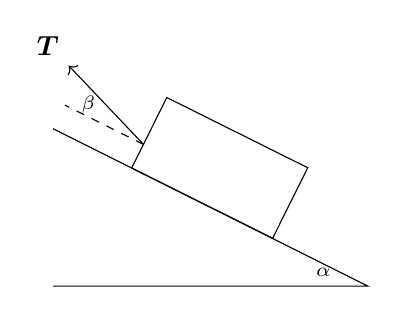
\begin{tikzpicture}
\draw (-2,0) -- (2,0) -- (-2,2);
\draw [rotate around={-26.47:(-1,1.5)}] (-1, 1.5) rectangle (1,2.5);
\draw [->] (-0.85,1.8) -- (-1.8,2.8);
\draw [dashed] (-0.85,1.8) -- (-1.85, 2.3);
\node [above left] at (1.65,0) {\({\scriptstyle\alpha}\)};
\node at (-1.55, 2.3) {\({\scriptstyle\beta}\)};
\node [above left] at (-1.8,2.8) {\(\vec T\)};
\end{tikzpicture}
\end{center}
A ship rests is on a slope held stationary by a light rope. What is the maximum tension \(T\) of the rope before the ship moves up the slope?

\subsubsection*{Method}
\begin{enumerate}
\item First draw a vector diagram:
\begin{center}
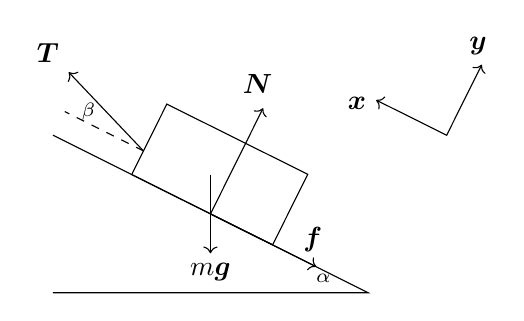
\begin{tikzpicture}
\draw (-2,0) -- (2,0) -- (-2,2);
\draw [rotate around={-26.47:(-1,1.5)}] (-1, 1.5) rectangle (1,2.5);
\draw [->] (-0.85,1.8) -- (-1.8,2.8);
\draw [dashed] (-0.85,1.8) -- (-1.85, 2.3);
\node [above left] at (1.65,0) {\({\scriptstyle\alpha}\)};
\node at (-1.55, 2.3) {\({\scriptstyle\beta}\)};
\node [above left] at (-1.8,2.8) {\(\vv T\)};
\draw [->] (0,1.5) -- (0, 0.5);
\draw [->, rotate around={-26.47:(0,1)}] (0,1) -- (0,2.5);
\draw [->, rotate around={-26.47:(0,1)}] (0,1) -- (1.5,1);
\node [above] at (0.6, 2.4) {\(\vv N\)};
\node [below] at (0,0.5) {\(m\vv g\)};
\node [above] at (1.3, 0.4) {\(\vv f\)};
\draw [<->, rotate around={-26.47:(3,2)}] (3,3) -- (3,2) -- (2,2);
\node [above] at (3.4,2.9) {\(\vv y\)};
\node [left] at (2.1, 2.4) {\(\vv x\)};
\end{tikzpicture}
\end{center}

Note friction is downhill as we want the maximum value \(T\) can take.
\item Identify vector equations and equations of motion (EOM):

Newton's second law:
\[m\vv a=m\vv g+\vv T+\vv N+\vv f\]
The ship is stationary so \(\vv a=\vv 0\) 
\item Choose a coordinate system and decompose vectors:
\[\vv N = N\vv y\]
\[\vv f = -f\vv x\]
\[m\vv g=mg(-\sin\alpha\vv x-\cos\alpha\vv y)\]
\[\vv T = T(\cos\beta\vv x+\si\beta\vv y)\]
\item Extract component equations
\begin{align*}
\vv x: &\quad -f-mg\sin\alpha+T\cos\beta=0\tag{14.1}\\
\vv y: &\quad T\sin\beta -mg\cos\alpha+N=0\tag{14.2}
\end{align*}
Also \(f\le\mu N\). Since we want the maximum \(T\) we take \(f=\mu N\)(14.3)
\item Solve

Substitute (14.3) in (14.1)
\[0=T\cos\beta-mg\sin\alpha-\mu N\tag{14.4}\]
\(\mu\cdot(14.2)+(14.4)\)
\[0=T(\mu\sin\beta+\cos\beta)-mg(\mu\cos\alpha+\sin\alpha)\]
\[T=mg\frac{\mu\cos\alpha+\sin\alpha}{\mu\sin\beta+\cos\beta}\]
\item Check
\begin{align*}
[\si{N}]&=[\si{kg}][\si{m.s^{-2}}]\\
[\si{kg.m.s^{-2}}]&=[\si{kg.m.s^{-2}}]\quad\checkmark
\end{align*}
\[
\begin{array}{l l l}
m\to 0 & T\to 0 & \checkmark\\
g\to 0 & T\to 0 & \checkmark\\
m\to \infty & T\to\infty & \checkmark\\
g \to \infty & T\to\infty & \checkmark\\
\alpha \to 0\text{ and }\beta\to \frac{\pi}{2} & T\to mg & \checkmark\\
\alpha\to 0\text{ and }\beta\to 0 & T\to mg\mu=\mu N=f&\checkmark\\
\end{array}
\]
\end{enumerate}

\section{Boxes and Pulleys on a Slope}

\begin{center}
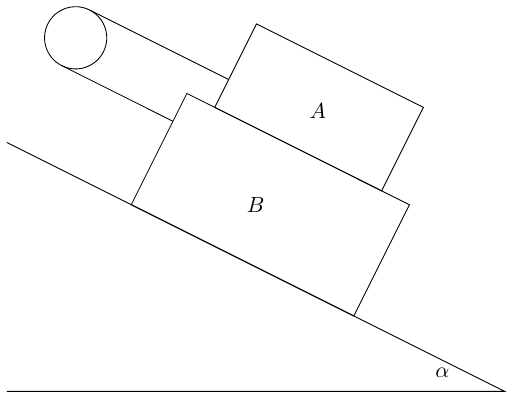
\includegraphics[scale=0.4]{BothBoxes}
\end{center}
Two boxes, box \(A\) mass \(m\) and box \(B\) mass \(M\) where \(m\ll M\). The boxes are connected by a light inextendable string which passes over a light, smooth pulley. All surfaces are made of the same material and the coefficient of kinetic friction is \(\mu\)

It is possible to show that the acceleration of box \(A\) has the same magnitude and opposite direction to the acceleration of box \(B\) by considering the length of the string \(L\).

\begin{center}
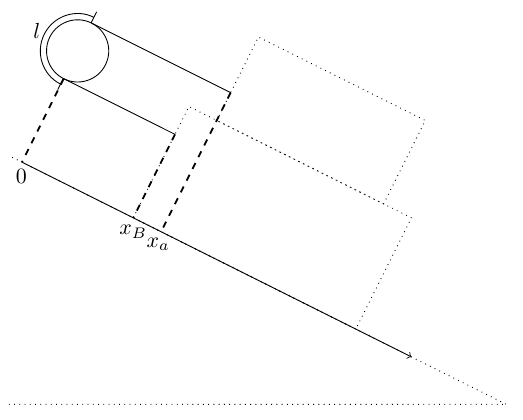
\includegraphics[scale=0.4]{StringLength}
\end{center}

The length of the string is a constant and the length of the string around the pulley is also a constant \(l\). The total length of the string is given by
\[L=x_A+x_B+l\]
Taking the second derivative with respect to time gives
\[\underbrace{\ddot L}_{=0}=\ddot x_A+\ddot x_B+\underbrace{\ddot l}_{=0}\]
Hence \(\ddot x_A=-\ddot x_B\)

We have three seperable systems. The first is box \(A\)

\begin{center}
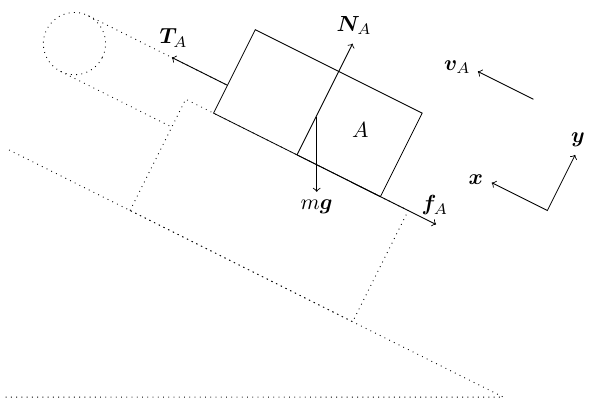
\includegraphics[scale=0.4]{BoxA}
\end{center}

\[\text{NII:}\qquad m\vv a=m\vv g+\vv T_A+\vv N_A+\vv f_A\]
\[\vv a=\ddot x\vh x\]
\[\implies\left\{
\begin{array}{cc}
\vv x: & m\ddot x=-mg\sin\alpha+T_A-f_A\\
\vv y: & 0 = -mg\cos\alpha+N_A
\end{array}
\right.\]
Also \(f_A=\mu N_A\)

Considering box B

\begin{center}
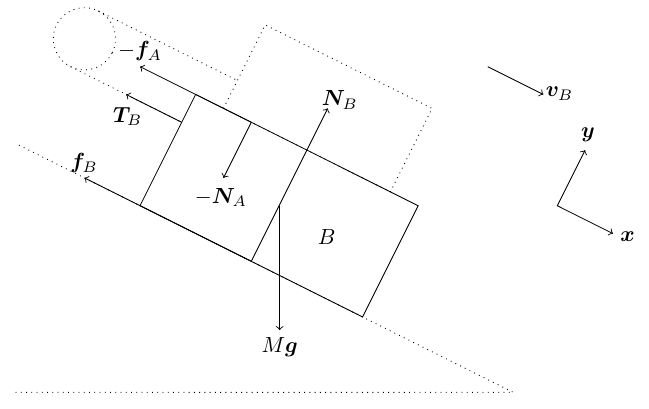
\includegraphics[scale=0.4]{BoxB}
\end{center}

\[\text{NII:}\qquad M\vv a=M\vv g+\vv T_B+\vv N_B+\vv f_B-\vv N_A-\vv f_A\]
\[\vv a=\ddot x\vh x\]
\[\implies\left\{
\begin{array}{cc}
\vv x: M\ddot x=Mg\sin\alpha-T_B-f_B-f_A\\
\vv y: 0=-Mg\cos\alpha+N_B-N_A
\end{array}
\right.\]
Also \(f_B=\mu N_B\)

Considering the  pulley

\begin{center}
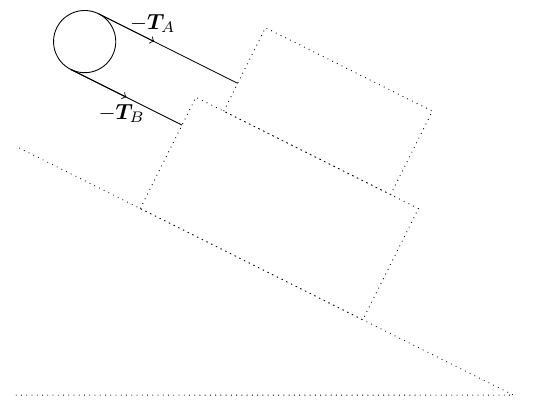
\includegraphics[scale=0.4]{Pulley}
\end{center}

\[\text{NII:}\qquad \vv T_A+\vv T_B=0\]
\[\implies T_A=T_B=T\]

Acceleration is constant. By eliminating contact forces we get
\[\implies\left\{
\begin{array}{c}
m\ddot x=T-mg(\sin\alpha+\mu\cos\alpha)\\
M\ddot x=Mg\sin\alpha-\mu(m+M)g\cos\alpha-\mu mg\cos\alpha-T
\end{array}
\right.\]
It is then possible to solve these DE for \(\ddot x\) and \(x\).

What if the pulley is rough?

If the pulley is rough then there will be friction between the rope and the pulley. How much friction can be calculated by considering a small length of rope.

\begin{center}
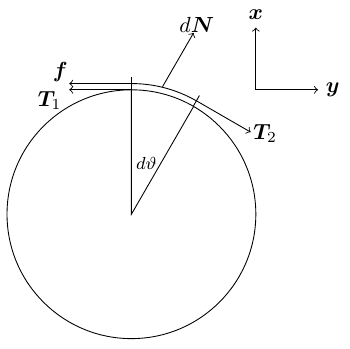
\includegraphics[scale=0.6]{RoughPulley}
\end{center}

In the case where \(T_2>T_1\) it is possible to write \(T_2=T_1+dT\) for some small amount \(0<dT\ll1\).
\[\vv T_1=T\vh x\]
\[\vv T_2=(T+dT)(\cos d\vartheta\vh x-\sin d\vartheta\vh y\]
For a rough enough pulley \(\ddot x=0\)
\[\text{NII: } \vv 0=\vv T_1+\vv T_2+d\vv N+d\vv f\]
\[\implies\left\{
\begin{array}{cc}
\vv x: & 0=(T+dT)\cos d\vartheta-df-T\\
\vv y: & 0=dN-(T+dT)\sin d\vartheta
\end{array}
\right.\]
\[df\le\mu dN\]
From the \(x\) components we get \(dt=df\) and from the \(y\) components we get \(dN=Td\vartheta\) by using the series expansions of sine. Combining all equations gives \(dN=\mu Td\vartheta\). This gives us the DE \(\frac 1T\dv T\vartheta=\mu\). Solving this gives \(T=T_0e^{\mu\vartheta}\) and since \(dT=df\) \(f=f_0e^{\mu\vartheta}\)

\part{Curvilinear motion}
\section{Polar Coordinates}

\subsection*{Cylindrical Polar Coordinates}

\begin{center}
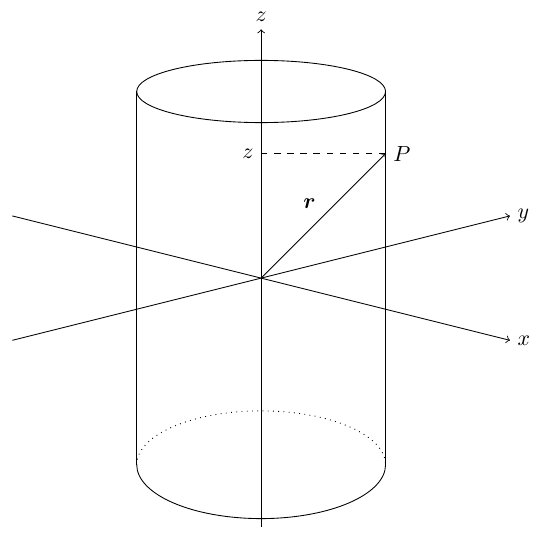
\includegraphics[scale=0.4]{CylindricalPolarCoordinates}
\end{center}
To describe a point on the cylinder shown we need its \(z\) coordinate, the radial distance from the \(z\) axis \(\varrho\) and the angle round the \(z\) axis \(\varphi\). By convention \(\varphi\) is measured from the positive \(x\) axis and increases counterclockwise. as shown below.

\begin{center}
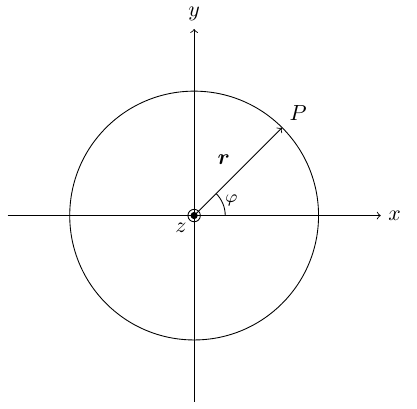
\includegraphics[scale=0.4]{PolarCoordinatesTopDown}
\end{center}

The natural domains of \(z,\varrho\) and \(\varphi\) are \(z,\varrho\in[0,\infty)\) and \(\varphi\in[0,2\pi)\).

We need two sets of transformation equations, one for the coordinate axis and one for the unit vectors. It can be seen from the diagram that the coordinates are given by
\[\left\{
\begin{array}{l}
x = \varrho\cos\varphi\\
y = \varrho\sin\varphi\\
z = z
\end{array}
\right.\iff\left\{
\begin{array}{l}
\varrho = \sqrt{x^2+y^2}\\
\varphi = \arctan\frac yx\\
z = z
\end{array}
\right.\]
The cylindrical polar coordinates unit vectors are \(\vh z\), \(\vh\varrho\) which is radial to the \(z\) axis and starts at the point, and \(\vh\varphi\) which is normal to \(\vh\varrho\) and tangental to the cylindar. It points in the direction in which \(\varphi\) increases.

\begin{center}
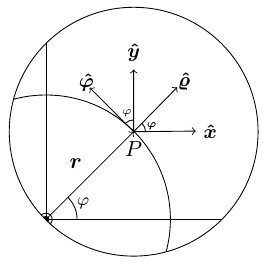
\includegraphics[scale=0.6]{CylindricalPolarUnitVectors}
\end{center}

It can be seen that the cylindrical polar unit vectors are just a rotation of the cartesian unit vectors about the \(z\) axis through an angle \(\varphi\).
\[\left\{
\begin{array}{l}
\vh x = \cos\varphi\vh\varrho-\sin\varphi\vh\varphi\\
\vh y = \sin\varphi\vh\varrho+\cos\varphi\vh\varphi\\
\vh z = \vh z
\end{array}
\right.\iff\left\{
\begin{array}{l}
\vh\varrho = \cos\varphi\vh x+\sin\varphi\vh y\\
\vh\varphi = -\sin\varphi\vh x+\cos\varphi\vh y\\
\vh z = \vh z
\end{array}
\right.\]
\[
\begin{pmatrix}
\vh\varrho \\ \vh\varphi \\ \vh z
\end{pmatrix}
=R_z(\varphi)
\begin{pmatrix}
\vh x \\ \vh y \\ \vh z
\end{pmatrix}
\iff
\begin{pmatrix}
\vh x \\ \vh y \\ \vh z
\end{pmatrix}
=R_z^T(\varphi)
\begin{pmatrix}
\vh\varrho \\ \vh\varphi \\ \vh z
\end{pmatrix}
\]
For a general point with position vector \(\vv r\)
\begin{align*}
\vv r &= x\vh x+y\vh y+z\vh z\\
&= \rho\cos\varphi(\cos\varphi\vh\rho-\sin\varphi\vh\varphi)+\varrho\sin\varphi(\sin\varphi\vh\varrho+\cos\varphi\vh\varphi)+z\vh z\\
&= \rho(\cos^2\varphi+\sin^2\varphi)\vh\varrho+\varrho(-\cos\varphi\sin\varphi+\sin\varphi\cos\varphi)\vh\varphi+z\vh z\\
&= \varrho\vh\varrho+z\vh z
\end{align*}
This shows that the choice of \(\varphi=0\) and hence the \(x\) axis is unimportant due to symmetry. This has the advantage of making a lot of problems easier but does mean we can't pin down the exact position of the point just give a circle that we know it is on.

\subsubsection*{Comments}
\begin{itemize}
\item \(\vh\varrho\times\vh\varphi=\vh z\) defines the right hand rule for cylindrical polar coordinates.
\item \(\vh\varrho,\vh\varphi\) and \(\vh z\) form a orthonormal base (ortho - all orthogonal, normal - all have length 1)
\item \(\varrho\) and \(z\) have dimension length
\item \(\varphi\) is dimensionless
\item \(\vh\varrho\) and \(\vh\varphi\) are time dependant as they change as the point moves
\end{itemize}

\subsection*{Spherical Polar Coordinates}

To describe a point on the surface of the sphere we need the radial distance from the origin \(r\), the ``latitude'' from the the positive \(z\) axis \(\vartheta\) and the ``longitude'' \(\varphi\), defined the same as with cylindrical polar coordinates.

Typical domains for these values are \(r\in[0,\infty),\vartheta\in[0,\pi]\) and \(\varphi\in[0,2\pi)\).

\begin{center}
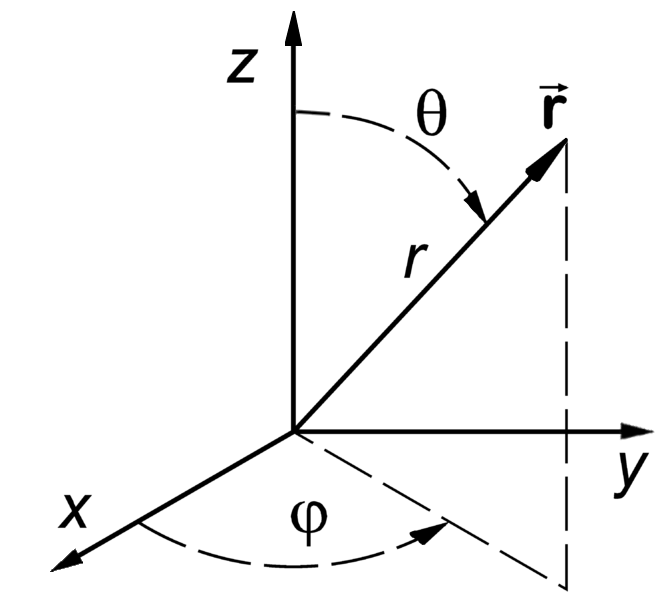
\includegraphics[scale=0.4]{SphericalPolarCoordinates}
\end{center}

It can be seen from the diagram that \(\varrho=r\sin\vartheta\). By substitiuting cartesian coordinates for cylindrical and then again for spherical we can get the coordinate transform equations
\[\left\{
\begin{array}{lll}
x & =\varrho\cos\varphi & =r\sin\vartheta\cos\varphi\\
y & =\varrho\sin\varphi & =r\sin\vartheta\sin\varphi\\
z & =z & =r\cos\vartheta
\end{array}
\right.\]

\section{Derivatives in Polar Coordinates}

The spherical coordinate unit vectors are \(\vh r,\vh\vartheta\) and \(\vh\varphi\). \(\vh r\) extends radialy from the origin. \(\vh\vartheta\) is tangental to the sphere and points from the \(z\) axis to the \(x,y\) plane. \(\vh\varphi\) is the same as in cylindrical polar coordinates. \(\vh r\times\vh\vartheta=\vh\varphi\) defines the right hand rule for this system.

\begin{center}
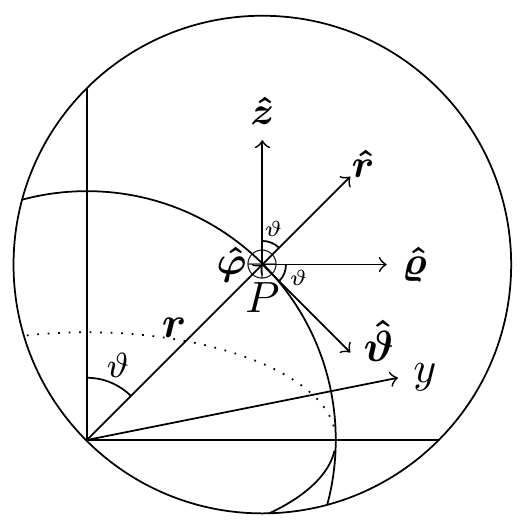
\includegraphics[scale=0.3]{SphericalPolarUnitVectors}
\end{center}

It can be seen that the spherical polar unit vectors are a rotation of the sylindrical polar unit vectors through an angle of \(\vartheta\). It is a positive rotation but in the diagram \(\vh\varphi\) is into the page so it looks like a clockwise rotation. The unit vectors are given as
\[\left\{
\begin{array}{l}
\vh r=\cos\vartheta\vh z+\sin\vartheta\vh\varrho\\
\vh\vartheta=-\sin\vartheta\vh z+\cos\vartheta\vh\varrho\\
\vh\varphi=\vh\varphi
\end{array}
\right.\iff\left\{
\begin{array}{l}
\vh z = \cos\vartheta\vh r-\sin\vartheta\vh\vartheta\\
\vh\varrho = \sin\vartheta\vh r+\cos\vartheta\vh\vartheta\\
\vh \varphi=\vh\varphi
\end{array}
\right.\]
\[R_\varphi(\vartheta)
\begin{pmatrix}
\vh z \\ \vh \varrho \\ \vh \varphi
\end{pmatrix}
=
\begin{pmatrix}
\cos\vartheta & \sin\vartheta & 0\\
-\sin\vartheta & \cos\vartheta & 0\\
0 & 0 & 1
\end{pmatrix}
\begin{pmatrix}
\vh z \\ \vh \varrho \\ \vh \varphi
\end{pmatrix}
=
\begin{pmatrix}
\vh r \\ \vh \vartheta \\ \vh \varphi
\end{pmatrix}
\]
\[R_z(\varphi)
\begin{pmatrix}
\vh x \\ \vh y \\ \vh z
\end{pmatrix}
=
\begin{pmatrix}
0 & 0 & 1\\
\cos\varphi & \sin\varphi & 0\\
-\sin\varphi & \cos\varphi & 0
\end{pmatrix}
\begin{pmatrix}
\vh x \\ \vh y \\ \vh z
\end{pmatrix}
=
\begin{pmatrix}
\vh \varrho \\ \vh \varphi \\ \vh z
\end{pmatrix}
\]
Let \(R=R_\varphi(\vartheta)R_z(\varphi)\)
\[R
\begin{pmatrix}
\vh x \\ \vh y \\ \vh z
\end{pmatrix}
=
\begin{pmatrix}
\sin\vartheta\cos\varphi & \sin\vartheta\sin\varphi & \cos\vartheta\\
\cos\vartheta\cos\varphi & \cos\vartheta\sin\varphi & -\sin\vartheta\\
-\sin\varphi & \cos\varphi & 0
\end{pmatrix}
\begin{pmatrix}
\vh x \\ \vh y \\ \vh z
\end{pmatrix}
=
\begin{pmatrix}
\vh r \\ \vh \vartheta \\ \vh \varphi
\end{pmatrix}
\]
Since \(R\) is a rotation matrix it is orthogonal so its inverse is \(R^T\)
We can use this to give the spherical polar unit vectors in terms of cartesian unit vectors
\[\left\{
\begin{array}{l}
\vh r = \sin\vartheta\cos\varphi\vh x+\sin\vartheta\sin\varphi\vh y+\cos\vartheta\vh z\\
\vh \vartheta = \cos\vartheta\cos\varphi\vh x+\cos\vartheta\sin\varphi\vh y-\sin\vartheta\vh z\\
\vh \varphi = -\sin\varphi\vh x+\cos\varphi y+0\vh z
\end{array}
\right.\iff\left\{
\begin{array}{l}
\vh x = \sin\vartheta\cos\varphi\vh r+\cos\vartheta\cos\varphi\vh \vartheta-\sin\varphi\vh \varphi\\
\vh y = \sin\vartheta\sin\varphi\vh r+\cos\vartheta\sin\varphi\vh \vartheta+\cos\varphi\vh \varphi\\
\vh z = \cos\vartheta\vh r-\sin\vartheta\vh \vartheta+0\vh\varphi
\end{array}
\right.\]
Let \(\vv r\) be a position vector

\begin{align*}
\vv r &= x\vh x+y\vh y+z\vh z\\
&= r\sin\vartheta\cos\varphi(\sin\vartheta\cos\varphi\vh r+\cos\vartheta\cos\varphi\vh\vartheta-\sin\varphi\vh\varphi)\\
&\hphantom{=}+r\sin\vartheta\sin\varphi(\sin\vartheta\sin\varphi\vh r+\cos\vartheta\sin\varphi\vh \vartheta+\cos\varphi\vh \varphi)\\
&\hphantom{=}+r\cos\vartheta(\cos\vartheta\vh r-\sin\vartheta\vh \vartheta)\\
&=(r\sin^2\vartheta\cos^2\varphi+r\sin^2\vartheta\sin^2\varphi+r\cos^2\vartheta)\vh r\\
&\hphantom{=}+(r\sin\vartheta\cos\vartheta\cos^2\varphi+r\sin\vartheta\cos\vartheta\sin^2\varphi-r\cos\vartheta\sin\vartheta)\vh\vartheta\\
&\hphantom{=}+(-r\sin\vartheta\cos\varphi\sin\varphi+r\sin\vartheta\sin\varphi\cos\varphi+r\cos\vartheta)\vh\varphi\\
&=r\vh r
\end{align*}
This shows that the choice of \(x\) and \(z\) axes is unimportant. However, we can't exactly specify a position in sperical polar coordinates since we would need to know \(\vh r\) and it is time dependant.

\subsection*{Time derivateives}

In cylinindrical coordinates \((\varrho,\varphi,z)\) a general position vector is given by
\[\vv r = \varrho\vh\varrho+z\vh z\]
The velocity vector is given by
\begin{align*}
\vv v&=\dv{\vh r}{t}\\
&=\diff t(\varrho\vh\varrho)+\diff t(z\vh z)\\
&=\dv{\varrho}{t}\vh\varrho+\varrho\dv{\vh\varrho}{t}+\dot z\vh z\\
\intertext{We can calculate \(\dot{\vh\varrho}\) by substituting in the cartesian coordinates}
\dv{\vh\varrho}{t}&=\diff t(\cos\varphi\vh x+\sin\varphi\vh y)\\
&=\dv{\cos\varphi}{t}\vh x+\dv{\sin\varphi}{t}\vh y\\
&=\dv{\cos\varphi}{\varphi}\dv{\varphi}{t}+\dv{\sin\varphi}{\varphi}\dv{\varphi}{t}\\
&=-\dot\varphi\sin\varphi\vh x+\dot\varphi\cos\varphi\vh y\\
&=\dot\varphi(-\sin\varphi\vh x+\cos\varphi\vh y)\\
&=\dot\varphi\vh\varphi\\
\intertext{\(\dot{\vh\varrho}\) has units of \si{s^{-1}} so we interpret it as angular velocity}
\vv v&=\dv{\varrho}{t}\vh\varrho+\varrho\dv{\varphi}{t}\vh\varphi+\dv{z}{t}\vh z\\
&=\dot\varrho\vh\varrho+\varrho\dot\varphi\vh\varphi+\dot z\vh z\\
\intertext{It is also possible to find the velocity vector in cylindrical coordinates}
\vv a&=\dv{\vv v}{t}\\
&=\diff t(\dot\varrho\vh\varrho+\varrho\dot\varphi\vh\varphi+\dot z\vh z)\\
&=\ddot\varrho\vh\varrho+\dot\varrho\dot{\vh\varrho}+\dot\varrho\dot\varphi\vh\varphi+\varrho\ddot\varphi\vh\varphi+\varrho\dot\varphi\dot{\vh\varphi}+\ddot z\vh z\\
\dot{\vh\varphi}&=\diff t(-\sin\varphi\vh x+\cos\varphi\vh y)\\
&=-\dot\varphi\cos\varphi\vh x-\dot\varphi\sin\varphi\vh y\\
&=-\dot\varphi\vh\varrho\\
\vv a&=(\ddot\varrho-\varrho\dot\varphi^2)\vh\varrho+(\varrho\ddot\varphi+2\dot\varrho\dot\varphi)\vh\varphi+\ddot z\vh z
\end{align*}

\subsection*{Circular motion}
Consider circular motion on the \(x,y\) plane with constant angular velocity, for a particle travelling on a circular path radius \(R\). This means that \(z=\) constant\(\implies\dot z=\ddot z=0\), \(\varrho=R=\) constant\(\implies\dot\varrho=\ddot\varrho=0\) and \(\omega=\dot\varphi=\) constant\(\implies\ddot\varphi=\alpha=0\).
\[\vv v=\varrho\dot\varphi\vh\varphi=R\omega\vh\varphi\]
This is tangental to the path and has constant magnitude as expected.
\[\vv a=-\varrho\dot\varphi^2\vh\varrho=-R\omega^2\vh\varrho\]
This is towards the center as expected.

Note that while using cylindrical and spherical polar coordinates cylindrical polar coordinates are \((\varrho,\varphi,z)\). When not using spherical polar coordinates it is common to use \((r,\vartheta,z)\) instead for cylindrical polar coordinates.

\section{Normal and Tangental Coordinates}

\begin{center}
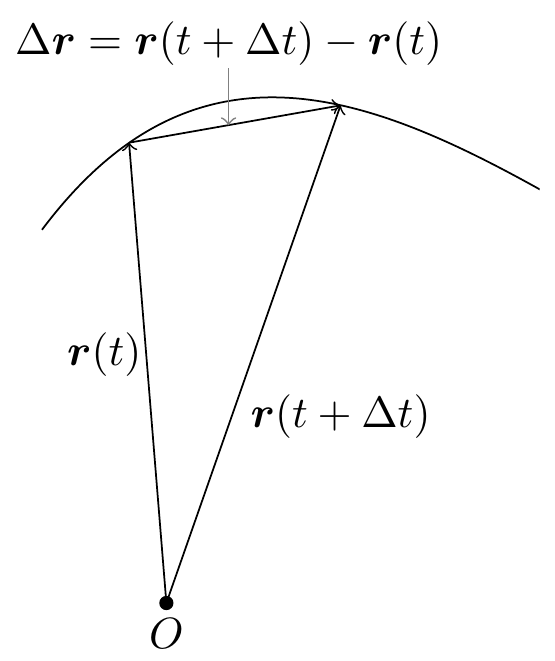
\includegraphics[scale=0.3]{PositionVectors}
\end{center}
This shows a path \(s\) in a plane. \(\vv r(t)\) is the position vectorof a particle travelling on the path at time \(t\). The velocity \(\vv v\) is given by
\[\vv v=\lim_{\Delta t\to0}\frac{\Delta\vv r}{\Delta t}=\lim_{\Delta t\to0}\frac{\vv r(t+\Delta t)-\vv r(t)}{\Delta t}=\dv{\vv r}{t}\]
A small element of the path \(d\vv r\) is given by
\[d\vv r=ds\ve t\]
Where \(ds\) is a small segment of the path and \(\ve t\) is a unit vector tangental to the path. Sometimes \(\ve t\) is denoted \(\vh t\). This gives us the relation
\[\ve t=\dv{\vv r}{s}\]
\[\implies\vv v=\dv{\vv r}{t}=\dv{\vv r}{s}\dv{s}{t}=v\ve t\]
\[\implies\vv a=\dv{\vv v}{t}=\diff t(v\ve t)=\dv vt\ve t+\dv{\ve t}{t}v\]
\(\displaystyle{\dv vt}=a_t\) is the magnitude of the tangental component of the acceleration vector and describes the rate of change of speed.
\[\ve t\cdot\ve t=1\]
\[\diff t(\ve t\cdot\ve t=\diff t1=0\]
Applying the product rule gives
\[2\ve t\cdot\dv{\ve t}{t}=0\]
\[\ve t\cdot\dv{\ve t}{t}=0\]
This means that \(\ve t\) is normal to \(\dv{\ve t}{t}\).
\[\dv{\ve t}{t}=\dv{\ve t}{ds}\dv st=v\dv{\ve t}{s}\]
Let \(\ve n=\vh n\) be a unit vector normal to the path
\[\ve n=\frac{\dv{\ve t}{s}}{\left|\dv{\ve t}{s}\right|}\]
\[\left|\dv{\ve t}{s}\right|=\kappa\]
\(\kappa\) is the curvature of the path
\[\dv{\ve t}{s}=\kappa \ve n\]
For a straight line \(\kappa =0\)
Let \(\varrho\) be the instantaneous radius of curvature.
\[\varrho=\frac{1}{\kappa}\]
For a straight line \(\varrho\to\infty\)
\[\ve n=\varrho\dv{\ve t}{s}\]
\[\vv a=\dv vt\ve t+\frac{v^2}{\varrho}\ve n\]
The normal term describes the rate of change of direction of \(\vv v\). 

By convention \(\ve n\) points in towards the center of the curve.

For a small arc of the cuve with arc length \(ds\), angle \(\vartheta\) and radius \(R\) we get
\[ds=Rd\vartheta\]
\[s=R\vartheta\]
\[s=\varrho\vartheta\]
\[\implies v=\dv st=\diff t(\varrho\vartheta)=\varrho\dv{\vartheta}{t}=\varrho\omega\]
This result comes from the product rule and the fact that \(\dot\varrho=0\). This is the result that we would expect for circular motion which is approximated by a curved path.
\[a_n=\frac{v^2}{\varrho}=\frac{1}{\varrho}(\varrho\dot\vartheta)^2=\varrho\omega^2\]
Which is the centripetal acceleration from circular motion, which is what we would expect since centripetal acceleration is tangental to the circle and inwards.

\begin{example}
\begin{center}
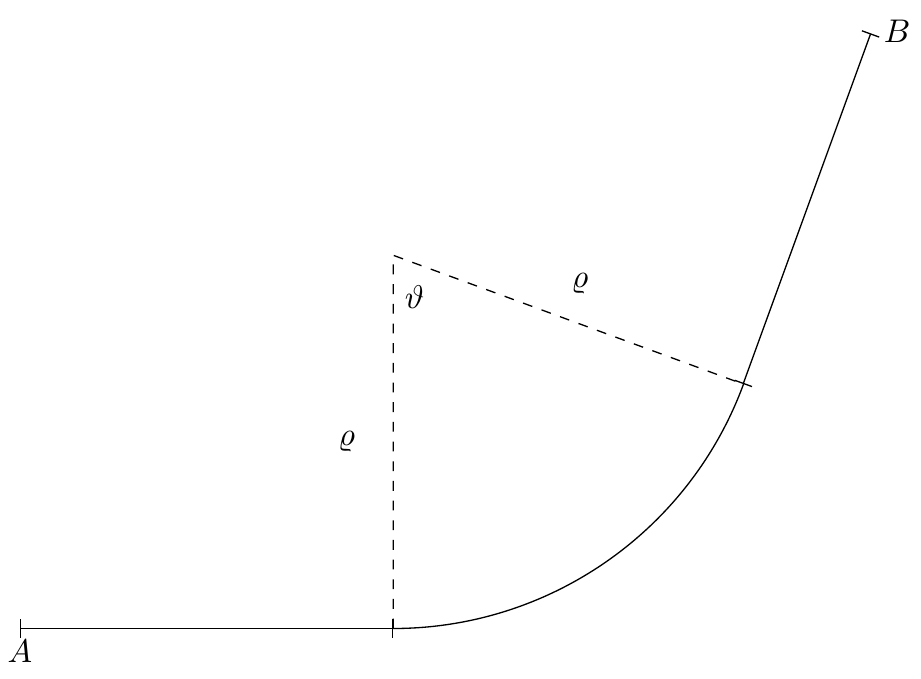
\includegraphics[scale=0.25]{StraightCurveStraight}
\end{center}

This path is made of two straight sections of length \(D\) and one arc angle \(\vartheta\) and radius \(\varrho\). A car travels along this path. At \(A\) it has speed \(v_A\) and at \(B\) it has speed \(v_B\). Its speed increases at a constant rate. Find \(|\vv a(t)|\).

\begin{enumerate}
\item Speed increases at a constant rate so \(a_t=\dv vt\) is a constant.

Total path length \(s=2D+\varrho\vartheta\)
\[\vv a=\dv vt\ve t+a_n\ve n\]
\[\dv vt=\dv vs\dv st=v\dv vs\]
\[\implies \int_A^Ba_t\,ds=\int_{v_A}^{v_B}v\,dv=\left[\frac{v^2}{2}\right]_{v_A}^{v_B}\]
\[a_t=\frac{v_B^2-v_A^2}{2(2D+\varrho\vartheta)}\]
\item Find \(s(t)\)
\[a_t=\dv vt\implies v(t)=v_A+a_tt\]
Let \(t=0\) at \(A\)
\[v=\dv st\implies\int_0^tv_A+a_tt\,dt=\int_{s_A}^{s_B}ds\]
\[s(t)=v_At+\frac12a_t\frac{t^2}{2}\]
\item Let the car be at the end of the first straight at \(t_1\) and at the end of the curve at t\(_2\). \(s(t_1)<D\implies |\vv a|=a_t\). \(D\le s(t_2)<D+\varrho\vartheta\implies\vv a=a_t\ve t+\frac{v^2}{\varrho}\ve n\) where \(v(t_1)=v_A+a_tt\).
\[|\vv a|=\sqrt{a_t^2+a_n^2}\]
\[D+\varrho\vartheta<s(t_1)<s\vartheta\implies\vv a=a_t\ve t\]
\end{enumerate}
\end{example}

\section{Ant on a Pipe}

\begin{center}
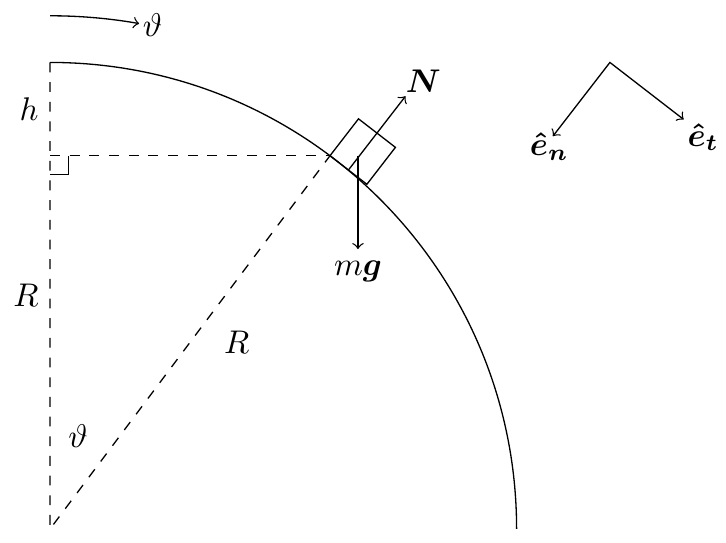
\includegraphics[scale=0.3]{AntOnPipe}
\end{center}

An ant of mass \(m\) sits on top of a wet cylindrical pipe radius \(R\). Suddenly the ant starts sliding down the pipe. Find the speed of the ant and the point at which it loses contact with the pipe.

The pipe is wet so we can ignore friction.
\begin{align*}
\text{NII: }m\vv a&=m\vv g+\vv N\\
\vv N&=-N\ve n\\
m\vv g&=mg(\sin\vartheta\ve t+\cos\vartheta\ve n)\\
\vv a&=\dv vt\ve t+\frac{v^2}{R}\ve n\\
\ve t:\quad m\dv vt&=mg\sin\vartheta\tag{19.1}\\
\ve n:\quad m\frac{v^2}{R}&=mg\cos\vartheta-N\tag{19.2}\\
\intertext{Find \(v(\vartheta)\)}
(19.2)\implies \dv vt&=g\sin\vartheta\\
v&=\dv st,\quad s=R\vartheta\\
v&=\dv st=R\dv \vartheta t=R\dot\vartheta\\
v^2&=R^2\dot\vartheta^2\\
\dv vt&=\diff t(R\dot\vartheta)=R\dv{\dot\vartheta}{t}=R\dv{\dot\vartheta}{\vartheta}\dv{\vartheta}{t}\\
\dv vt&=R\dot\vartheta\dv{\dot\vartheta}{t}=g\sin\vartheta\\
\dot\vartheta\dv{\dot\vartheta}{t}&=\frac{g}{R}\sin\vartheta\\
\int_{\vartheta(0)}^{\vartheta(t)}\dot\vartheta\,d\dot\vartheta&=\frac{g}{R}\int_{\vartheta(0)}^{\vartheta(t)}\sin\vartheta\,d\vartheta\\
\intertext{Where \(\vartheta(t)<\vartheta_c\), which is the point at which the ant loses contact with the cylinder, and \(\vartheta(0)=0\)}
\frac{\dot\vartheta^2}{2}&=\frac{g}{R}[-\cos\vartheta]_0^{\vartheta}=\frac{g}{R}(-\cos\vartheta)\\
\implies v^2&=2gR(1-\cos\vartheta)\\
\cos\vartheta&=\frac{R-H}{R}=1-\frac{h}{R}\\
\implies v^2&=2gR\left(1-1+\frac{h}{R}\right)=2gh\\
K&=\frac{mv^2}{2}=U=mgh\\
\implies v^2&=2gh\\
\intertext{Energy and forces agree, this is a good sign.}
\intertext{Consider motion in a straight line along the \(x\) axis. This means \(\vv F=m\vv a\), \(\vv v=v\vh x\) and \(\vv a=\dv vt\vh x\). Let \(\vv F\) be a force that is independant of \(t\) and \(\vv v\).}
m\dv vt&=F(x)\\
m\dv vx\dv xt&=F(x)\\
m\dv vx v&=F(x)\\
m\int_{v_1}^{v_2} v\,dv&=\int_{x_1}^{x_2}F(x)\,dx\\
m\left[\frac{v^2}{2}\right]_{v_1}^{v_2}&=\int_{x_1}^{x_2}F(x)\,dx\\
\frac{mv_2^2}{2}-\frac{mv_1^2}{2}&=\int_{x_1}^{x_2}F(x)\,dx\\
\Delta K&=W
\intertext{For more general motion}
\underbrace{\frac{mv_2^2}{2}}_{=T_2}-\underbrace{\frac{mv_1^2}{2}}_{=T_1}&=\underbrace{\int\vv F\cdot d\vv r}_{=W}\\
\intertext{Define \(U(x)\) such that \(F(x)=-\dv Ux\)}
\int_{x_1}^{x_2}F(x)\,dx&=\int_{x_1}^{x_2}-\dv Ux\,dx=-U_2+U_1\\
T_2-T_1&=U_1-U_2\\
U_1+T_1&=U_2+T_2=E\\
\intertext{\(E\) is the total mechanical energy. All forces are conservative so energy at the start is equal to energy at the end.}
\intertext{Alternate solution using energy instead of forces, apply the energy principal of word and kinetic energy}
\frac{mv_2^2}{2}-\underbrace{\frac{mv_1^2}{2}}_{=0}=&\int\vv F\cdot d\vv r\\
\frac{mv^2}{2}&=\int\vv F\cdot d\vv r\\
\vv F&=(mg\cos\vartheta-N)\ve n+mg\sin\vartheta\ve t\\
d\vv r&=ds\ve t\\
\vv F\cdot d\vv r&=mg\sin\vartheta ds\\
&=mgR\sin\vartheta d\vartheta\\
\frac{mv^2}{2}&=\int_{\vartheta_1}^{\vartheta_2}\sin\vartheta\, d\vartheta\\
\intertext{The same result follows that \(v^2=2gh\)}
\intertext{Find the critical angle \(\vartheta_c\) where the ant loses contact with the cylinder.}
N(\vartheta_c)&=0\\
(19.1)\implies N(\vartheta_c)&=mg\cos\vartheta-\frac{mv^2}{R}=0\\
g\cos\vartheta_c&=\frac{v^2}{R}=2g(1-\cos\vartheta_c)\\
\cos\vartheta_c&=2(1-\cos\vartheta_c)\\
\cos\vartheta_c&=\frac 23\\
\vartheta_c&=\arccos\frac 23
\end{align*}

\part{Second order ODE}

\section{Simple Harmonic Motion}

Consider a mass \(m\) attached to a spring \(k\), unextended length \(L\) where \(m,k,L\in\bb R\) and \(m,k,L>0\). If the mass is allowed to drop slowly it will reach an equilibrium point \(x_0\) where the spring holds it still.
\[\text{NII}:\quad m\vv a=m\vv g+\vv F_k\]
If we define \(x\) direction as vertical downwards then decomposing the vectors gives us
\begin{align*}
m\vv g&=mg\vh x\\
\vv F_k&=-F_k\vh x\\
\vv a&=\ddot x\vh x\\
\intertext{At \(x_0\) \(\vv a=\vv 0\) since it is at equilibrium.}
0&=mg-kx_0\\
\frac{mg}{k}&=x_0\\
\end{align*}

If we consider small oscillations about \(x_0\)  then \(x\) ranges across \(x_0\pm\Delta x\) where \(\Delta x\ll 1\). Since \(x_0\) is a constant its time derivative is 0.
\begin{align*}
\ddot x&=\ddot{\Delta x}\\
m\ddot{\Delta x}&=mg-k(x_0+\Delta x)\\
&=mg-\frac{mg}{k}kx_0-k\Delta x\\
\ddot{\Delta x}&=-\frac{k}{m}\Delta x
\end{align*}
If we choose \(x_0=0\) since \(x=\Delta x- x_0\) we get \(x=\Delta x\implies \ddot x=-\frac{k}{m}x\) where \(x\ll 1\).

Let \(\frac{k}{m}=\omega^2\implies \ddot x=-\omega^2 x\).

This gives a linear, second order ODE which is solved by \(x(t)\) where \(\ddot x(t)=-\omega^2 x(t)\). For \(A,B\in\bb C\) one solution is
\begin{align*}
x(t)&=A\sin\omega t+B\cos\omega t\\
\dot x(t)&=\omega A\cos\omega t-\omega B\sin\omega t\\
\ddot x(t)&=-\omega^2A\sin\omega t-\omega^2B\cos\omega t\\
&=-\omega^2(A\sin\omega t+B\cos\omega t)\\
&=-\omega^2x(t)
\end{align*}
The units of \(\omega\) are \si{s^{-1}} so we interpret it as angular frequency.

The period of oscillation \(T\) is given by \(\omega T=2\pi\implies T=2\pi\sqrt{\frac{m}{k}}\)

Let \(x(t)=A\sin\omega t\). \(\vv F(x)=-kx\vh x\), \(d\vv r=dx\vh x\)
\[U(x)=-\int\vv F\cdot d\vv r=-\int -kx\vh x\cdot dx\vh x=k\int x\,dx=\frac{kx^2}{2}+u_0\]
\(u_0\) is a constant of integration. Usually boundary conditions are chosen such that \(u_0=0\). Plotting the function of \(U\) against \(x\) we get a parabola, the minimum of the parabola is at \(x_0\) which is 0 if \(u_0=0\). Using this we can say that any system will oscillate if there is a linear restoring force \(F=-kx\) where \(k>0\) and teh potential takes the form \(\frac{kx^2}{2}+u_0\). All other results follow from this.

If we consider a system with potential \(U(x)\) if \(U(x_0)\) is a minimum then the system will oscillate around this point for sufficently small \(\Delta x\). It is possible to approximate \(U(x)\) about \(x=x_0\) using a taylor series:
\[U(x)=U(x_0)+U'(x_0)(x-x_0)+\frac{U''(x_0)}{2}(x-x_0)^2+\mathcal{O}(x^3)\]
It is possible to choose what point to call \(U=0\) so that \(U(x_0)=0\). Since we are expanding about a stationary point we know \(U(x_0)=0\). This leaves us with
\[U(x)\approx \frac{U''(x_0)}{2}x^2\]
Since it is a minimum we know that \(U''(x_0)>0\). Let \(k=U''(x_0)\implies U(x)\approx\frac{kx^2}{2}\implies m\ddot x=-kx\implies x=A\sin\omega t+B\cos\omega t\). Where \(\omega^2=\frac{U''(x_0)}{m}\) and \(T=2\pi\sqrt{\frac{m}{U''(x_0)}}\)

A minimum is a stable position of equilibrium as after a small displacement \(\Delta x\) it will return to the minimum. At a maximum the above expansion still holds but now \(U''(x_0)<0\implies k<0\implies m\ddot x=kx\). There are no oscillations.

\section{Damped Motion}

In this course we will consider only second order, linear, homogeneous ODE with constant coefficents, such as
\[\dv[2]{x}{t}+2b\dv xt + ax=0\tag{21.1}\]
where \(a\) and \(b\) are constants  and \(x=x(t)\). This is linear in \(x\) and all its derivatives. If \(b=0\) then this is the same as simple harmonic motion for \(a\ge 0\) and exponential for \(a<0\).

The solution \(x(t)\) is a function. This means that it must be (for this course) a combination of exponetiation, logarithms, sine/cosine and polynomials. Exponentials, logarithms and sine/cosine can be expressed as \(e^{\lambda t}\) for \(\lambda\in\bb C\). If \(\lambda\in\bb C\backslash\bb R\) then it is a combination of sine and cosine. If \(\lambda\in\bb R\) then it is a combination of exponentials and logarithms.

We make the anzatz that \(x(t)=Ce^{\lambda t}\) where \(C\) and \(\lambda\) are constants.
\begin{align*}
\dot x(t)&=C\lambda e^{\lambda t}=\lambda x(t)\\
\ddot x(t)&=C\lambda^2e^{\lambda t}=\lambda^2 x(t)
\end{align*}
If we substitute this into (21.1) we get
\[x(t)(\lambda^2+2b\lambda+a)=0\]
\(x(t)=0\) is a trivial solution. If \(x(t)\ne 0\) then we get the non trivial solutions given by
\[\lambda^2+2b\lambda+a=0\]
\[\implies \lambda=-b\pm\sqrt{b^2-a}\]
\[\implies\left\{
\begin{array}{c}
\lambda_1=-b+\sqrt{b^2-a}\\
\lambda_2=-b-\sqrt{b^2-a}
\end{array}
\right.\]
If \(b^2\ne a\) then
\[x(t)=C_1e^{\lambda_1t}+C_2e^{\lambda_2t}\]
where \(C_1,C_2\) are constants and \(\lambda_1,\lambda_2\) are as above.

If \(b^2<a\) then \(\sqrt{b^2-a}=\sqrt{-(a-b^2)}=i\sqrt{a-b^2}=i\omega\) where \(\omega=\sqrt{a-b^2}\in\bb R\). This means that the solutions are
\[x(t)=e^{-bt}[C_1e^{i\omega t}+C_2e^{-i\omega t}]=e^{-bt}[A\sin\omega t+B\cos\omega t]\]
where \(A,B\) are constants. Oscillations occur here but they are damped by the \(e^{-bt}\) term which causes the amplitude to decay to 0. This is called underdamped motion.

If \(b^2>a\) then \(\sqrt{b^2-a}=\gamma\in\bb R\). This means the solutions are
\[x(t)=e^{-bt}[C_1e^{\gamma t}+C_2e^{-\gamma t}]=e^{-bt}[A\sinh\gamma t+B\cosh\gamma t]\]
There are no oscillations, instead \(x\) just tends towards 0. This is called overdamped motion.

If \(b^2=a\) then \(x(t)=Ce^{-bt}\). There is only one solution. We have to modify our anzatz to contain a polynomial \(p(t)\) to get all solutions. The modified anzatz is
\[x(t)=p(t)e^{-bt}\]
\begin{align*}
\dot x(t)&=\dot pe^{-bt}+p(-b)e^{-bt}=e^{-bt}[\dot p-bp]\\
\ddot x(t)&=-be^{-bt}(\dot p-bp)+e^{-bt}(\ddot p-b\dot p)=e^{-bt}[\ddot p-2b\dot p+b^2p]
\end{align*}
Substituting this into (21.1) gives
\[e^{-bt}[(\ddot p-2b\dot p+b^2p)+2b(\dot p-bp)+ap]=0\]
\[e^{-bt}[\ddot p+p\underbrace{(a-b^2)}_{=0}]=0\]
\[\underbrace{e^{-bt}}_{>0}\ddot p=0\]
\[\implies \ddot p=0\]
This can only happen if all terms in \(p\) of order \(3\) or higher are 0.
\begin{align*}
\dv[2]pt&=0\\
\int\dv[2]pt\,dt&=\int 0\, dt\\
\dv pt&=0t+C_2\\
&=C_2\\
\int \dv pt\,dt&=\int C_2\,dt\\
p&=C_2t+C_1
\end{align*}
So an anzatz of \(x(t)=(C_1+C_2t)e^{\lambda t}\) will give us the solutions
\[x(t)=C_1e^{-bt}+C_2te^{-bt}\]
This gives no oscillations and decays quickly to 0. This is called criticaly damped motion.
\end{document}
















